\documentclass[letterpaper, 12pt]{article}
\usepackage[spanish, es-tabla]{babel} %%Paquete español para mac
\usepackage[utf8]{inputenc} %% Para unicode
\usepackage{graphicx} %% Para incluir figuras
\usepackage{ifpdf}
\usepackage{blindtext}
\DeclareGraphicsExtensions{.pdf}
\usepackage{fullpage}
\setcounter{totalnumber}{5}
\renewcommand{\textfraction}{0.1}
\usepackage[cmex10]{amsmath}
\usepackage{amssymb}
\usepackage{float}
\decimalpoint
\usepackage{url}
\usepackage{hyperref}
\usepackage{subcaption}
\hypersetup{colorlinks=false,bookmarksopen=true,linkbordercolor={1 1 1}}
\newcommand{\rfigura}[1]{Fig.\ref{#1}} %% redefine las figuras
\newcommand{\rtabla}[1]{Tabla \ref{#1}} %% redefine las tablas
\usepackage{enumerate} %% Paquete ara generar listas enumeradas
\usepackage{amsmath}
\usepackage{amssymb}
\usepackage{amsfonts}
\usepackage{graphicx}
\usepackage[table,xcdraw]{xcolor}
\usepackage{url}
\usepackage{fancyhdr}
\usepackage{float}
\usepackage{wrapfig}
\usepackage{enumerate}
\usepackage{titlesec}
\usepackage{vmargin}
\usepackage[export]{adjustbox}
\usepackage{imakeidx}
\usepackage{biblatex} %Imports biblatex package
\addbibresource{sample.bib} %Import the bibliography file


\usepackage{xcolor}
\usepackage{listings}%Para incluir archivos de codigo
\definecolor{codegreen}{rgb}{0,0.6,0}
\definecolor{codegray}{rgb}{0.5,0.5,0.5}
\definecolor{codepurple}{rgb}{0.58,0,0.82}
\definecolor{backcolour}{rgb}{0.95,0.95,0.92}

\lstdefinestyle{mystyle}{
    backgroundcolor=\color{backcolour},   
    commentstyle=\color{codegreen},
    keywordstyle=\color{magenta},
    numberstyle=\tiny\color{codegray},
    stringstyle=\color{codepurple},
    basicstyle=\ttfamily\footnotesize,
    breakatwhitespace=false,         
    breaklines=true,                 
    captionpos=b,                    
    keepspaces=true,                 
    numbers=left,                    
    numbersep=5pt,                  
    showspaces=false,                
    showstringspaces=false,
    showtabs=false,                  
    tabsize=2
}
\lstdefinestyle{python}
{
    style=shared,
    language={Python},
    %alsolanguage={[Sharp]C},
    basicstyle=\small\tt,
    keywordstyle=\color{blue},
    commentstyle=\color[rgb]{0.13,0.54,0.13},
    backgroundcolor=\color{cyan!10},
    morekeywords={
        Console,
        WriteLine,
        int,
    },
}
\lstset{style=mystyle}
\usepackage{marvosym}
\setlength{\parindent}{0pt}

\begin{document}

%%%%%%%%%%%%%%%%%%%%%%%%%%
%%%%%%   ENCABEZADO  %%%%%
%%%%%%%%%%%%%%%%%%%%%%%%%%
\vspace*{-1cm}
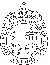
\includegraphics[width=2cm]{logo.pdf}
\vspace*{-2cm}

\hspace*{2cm}
 \begin{tabular}{l}
  {\ Pontificia Universidad Católica de Chile}\\
  {\ Escuela de Ingeniería}\\
  {\ Departamento de Ingeniería Eléctrica}\\
  {\ IEE2473 – Laboratorio de electrónica analógica y digital}\
 \end{tabular}
 \hfill 
\vspace*{1mm}
\begin{center}
{\Large\bf Experiencia 1}\\
\vspace*{1mm}
{\bf Grupo 24}\\
{\bf Juan Pablo Navarro - Tomas Infante}\\
\vspace*{1mm}
\end{center}
\hrule\vspace*{2pt}\hrule
% ***********************************************
% ***********************************************
\section{Trabajo Previo.}
\begin{figure}[H]
\centering
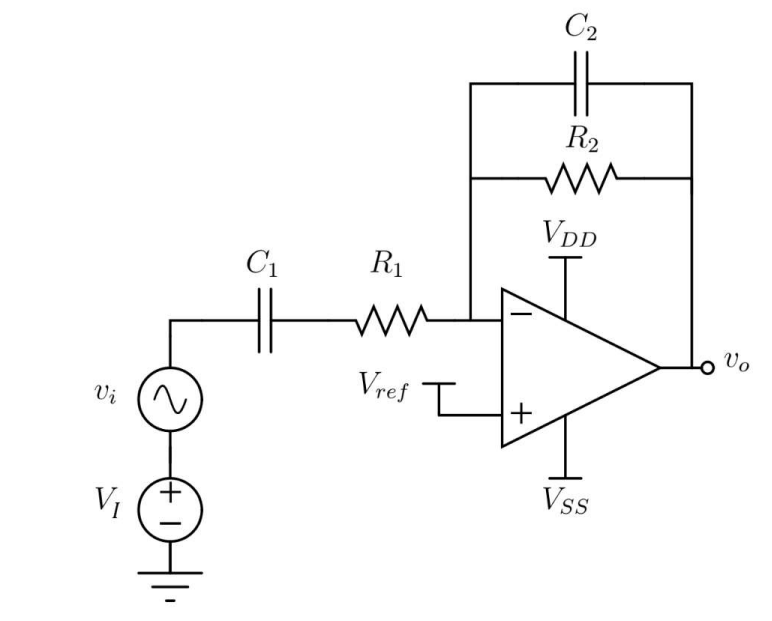
\includegraphics[width=0.7\textwidth]{Circuito_Acondicionador.png}
\label{Circuito Acondicionador}
\end{figure}
\subsection{Acodicionamiento de la señal}

1. Para calcular \(v_o\) en funcion de \(v_i\) y \(V_{ref}\) lo harmos por superposicion, entendiendo que el offset que entrega \(V_I\) tiene ganancia cero ya que el capacitor \(C_1\) elimina el offset y que \(V_{ref}\) se remplica en \(v_o\). Por lo tanto podemos hacer el analisis dejeando de lado el DC. Planteamos la ecuacion de nodo:
\[
\frac{-v_o}{\frac{1}{sC_2}\parallel R_2}= \frac{v_i}{R_1+\frac{1}{sC_1}}
\]
Operamos:
\[
\frac{(1+sC_2R_2)-v_o}{R_2}= \frac{v_isC_1}{1+sC_1R_1}
\]
\[
v_o= -\frac{v_isC_1R_2}{(1+sC_1R_1)(1+sC_2R_2)}
\]
Le sumamos la componente DC por superposcicion:
\[
v_o = V_{ref} - v_i \left[\frac{sC_1R_2}{(1+sC_1R_1)(1+sC_2R_2)}\right]
\]\\
2. En banda de interes el capacitor \(C_1\) opera como cortocircuito y \(C_2\) opera como circuito abierto. En tal caso las ecuaciones del circuito pasan a ser (En AC):
\[
\frac{-v_o}{R_2}= \frac{v_i}{R_1}
\]
\[
v_o= -\frac{R_2}{R_1}v_i
\]
Agregando la componente DC, queda:
\[
v_o = V_{ref}-v_i\frac{R_2}{R_1}
\]\\
3. Si \(C_2\) esta como circuito abierto las ecuaciones se reducen a (En AC):
\[
\frac{-v_o}{R_2}= \frac{v_i}{\frac{1}{sC_1}+R_1}
\]
\[
v_o =-\frac{v_isC_1R_2}{(1+sC_1R_1)}
\]
Agregamos la componente DC:

\[
v_o = V_{ref} - v_i \left[\frac{sC_1R_2}{(1+sC_1R_1)}\right]
\]
Como \(V_{ref}\) es un offset DC no genera desfase en la salida. Por lo tanto el analisis de desfase se hace en base a la funcion de tranferencia entre \(v_{o}\) sobre \(v_{i}\). Es decir:
\[
\frac{v_o}{v_i}=-\frac{sC_1R_2}{(1+sC_1R_1)}
\]
Donde:
\[
\phi_1(\omega) =\angle\left(-\frac{sC_1R_2}{(1+sC_1R_1)}\right)
\]
\[
\phi_1(\omega)=-90\text{°} -\arctan\left(\omega C_1 R_1\right)
\]
Equivalentemente:
\[
\phi_1(f)=-90 \text{°}  -\arctan\left(2\pi f C_1 R_1\right)
\]
4. Si \(C_1\) esta como cortocircuito las ecuaciones que deccriben el circuito son:
\[
\frac{-v_o(1+sC_2R_2)}{R_2}= \frac{v_i}{R_1}
\]
\[
v_o= -\frac{v_iR_2}{(1+sC_2R_2)R_1}
\]
Sumamos la componente DC por superposicion.
\[
v_o= V_{ref}-\frac{v_iR_2}{(1+sC_2R_2)R_1}
\]
Como \(V_{ref}\) es un offset DC no genera desfase en la salida. Por lo tanto el analisis de desfase se hace en base a la funcion de tranferencia entre \(v_{o}\) sobre \(v_{i}\). Es decir:
\[
\frac{v_o}{v_i} = -\frac{R_2}{(1+sC_2R_2)R_1}
\]
Donde:
\[
\phi_2(\omega) =\angle\left(-\frac{R_2}{(1+sC_2R2)R_1}\right)
\]
\[
\phi_2(\omega)=180\text{°} -\arctan\left(\omega C_2R_2 \right)
\]
Equivalentemente:
\[
\phi_2(f)=180\text{°} -\arctan\left(2\pi f C_2R_2 \right)
\]\\
5. Los capacitores electrolíticos ofrecen valores de capacitancia elevados pero presentan mayor tolerancia y son polarizados. Los capacitores cerámicos poseen menor capacitancia, son no polarizados y tienen mejor respuesta en altas frecuencias.
En el circuito propuesto, \(C_1\) requiere una capacitancia mayor para implementar el filtro pasa-altos cercano a 1 Hz, por lo que es más conveniente usar un capacitor electrolítico. En cambio, \(C_2\) tiene menor capacitancia y opera a frecuencias más altas, por lo que es más adecuado un capacitor cerámico.\\

6. Lo primero es evaluar la ganacia en banda pasante. Se desea acondicionar una señal de entrada que varía entre $3\,V$ y $10\,V$ al rango de $0\,V$ a $3.3\,V$.\\
Ya calculamos en 2. que (para la parte AC):
\[
v_o =-\frac{R_2}{R_1}v_i
\]
Esta expresión se puede comparar con una relacion lineal de la forma
\[
v_o = av_i
\]
Donde
\[
a = -\frac{R_2}{R_1}
\]
Para cumplir con las especificaciones del sistema se imponen las siguientes condiciones:
\[
v_i = 3V \rightarrow v_o = 0V
\]
\[
v_i = 10V \rightarrow v_o = 3.3V
\]
Sustituyendo en la ecuación del circuito:
\[
0 =  -\frac{R_2}{R_1}(3)
\]
\[
3.3 =-\frac{R_2}{R_1}(10)
\]
Restando ambas ecuaciones se obtiene
\[
3.3 = -\frac{R_2}{R_1}(7)
\]
\[
\frac{R_2}{R_1} = -\frac{3.3}{7}
\]
\[
\frac{R_2}{R_1} \approx -0.471
\]
En magnitud,
\[
\left|\frac{R_2}{R_1}\right| \approx 0.471
\]
Para obtener $V_{ref}$ tenemos en cuenta que en banda pasante se replica su valor en \(v_o\). Por lo tanto solo debemos fijarlo en el valor central entre \(0\,\)V y \(3.3\,\)V
\[
V_{ref} = \frac{3.3}{2}= 1.65\,\text{V}
\]
Finalmente, el diseño debe cumplir:
\[
\frac{R_2}{R_1} \approx 0.471
\]
\[
V_{ref} = 1.65\,\text{V}
\]
Obtenida la relacion entre \(R_1\) y \(R_2\). Solo queda cumplir el requerrimiento de: 
\begin{itemize}
    \item Ancho de banda menor o igual \(1\, \text{Hz}-400\, \text{Hz}\)
    \item Magnitud del desfase en los extremos
de la banda \(\approx 15\)° en relacion con el desfase en el centro de la banda \(20\) Hz
\end{itemize}
Debemos encontrar a que frecuencias tenemos \(\approx 15\)° respecto al desfase a los \(20\) Hz, sabemos que las frecuencias de corte cumplen:
\[
f_{c,\,bajo} = \frac{1}{2\pi C_1R_1}\quad  \longrightarrow\quad C_1 R_1 = \frac{1}{2\pi f_{c,\,bajo} }
\]
\[
f_{c,\,alto} = \frac{1}{2\pi C_2 R_2} \quad \longrightarrow \quad 
C_2 R_2 = \frac{1}{2\pi f_{c,\,alto} }
\]
Usando las ecuaciones obtenidas en 3 y en 4:
\[
\phi_1(f)=-90 \text{°}  -\arctan\left(2\pi f C_1 R_1\right)
\]
\[
\phi_2(f)=180\text{°} -\arctan\left(2\pi f C_2R_2 \right)
\]
Reemplazamos:
\[
\phi_1(f)=-90 \text{°}  -\arctan\left(\frac{f}{f_{c,\, bajo}}\right)
\]
\[
\phi_2(f)=180\text{°} -\arctan\left(\frac{f}{f_{c,\, alto}}\right)
\]
Ahora queda encontrar las frecuencias de corte para que se cumpla:
\[
|\phi_1(20)-\phi_1(1)| \approx 15\, \text{°}
\]
\[
|\phi_2(400)-\phi_2(20)| \approx 15\, \text{°}
\]
Lo que se traduce en:
\[
\left|-\arctan\left(\frac{20}{f_{c,\,bajo}}\right)+ \arctan\left(\frac{1}{f_{c,\,bajo}}\right)\right| \approx 15 \text{°}
\]
\[
\left|-\arctan\left(\frac{400}{f_{c,\,alto}}\right)+ \arctan\left(\frac{20}{f_{c,\,alto}}\right)\right| \approx 15 \text{°}
\]
Donde resolviendo con un programa llegamos a que las frecuencias de corte hay que ponerlas en:
\[
f_{c,\,bajo} = 0.283\,\text{Hz}
\]
\[
f_{c,\, alto} = 1412.51 \, \text{Hz}
\]
Obtenidas las frecuncias de corte, podemos ahora calcular los valores de \(C_1\), \(C_2\), \(R_1\) y \(R_2\).
\[
C_1 R_1 = \frac{1}{2\pi f_{c,\,bajo} } \quad \longrightarrow \quad C_1R_1 \approx 0.5624
\]
\[
C_2 R_2 = \frac{1}{2\pi f_{c,\,alto} } \quad \longrightarrow \quad C_2R_2 \approx 1.125\cdot 10^{-4}
\]
Asumamos \(R_1 = 100\,\text{k}\Omega\). En tal caso:
\[
R_2 = 47.1\,\text{k}\Omega \quad C_1 = 5.62\cdot 10 ^{-6}\, \text{F} \quad C_2 = 2.388\cdot 10^{-9}\, \text{F}
\]\\
8. Graficamos el diagrama de Bode
\begin{figure}[H]
\centering
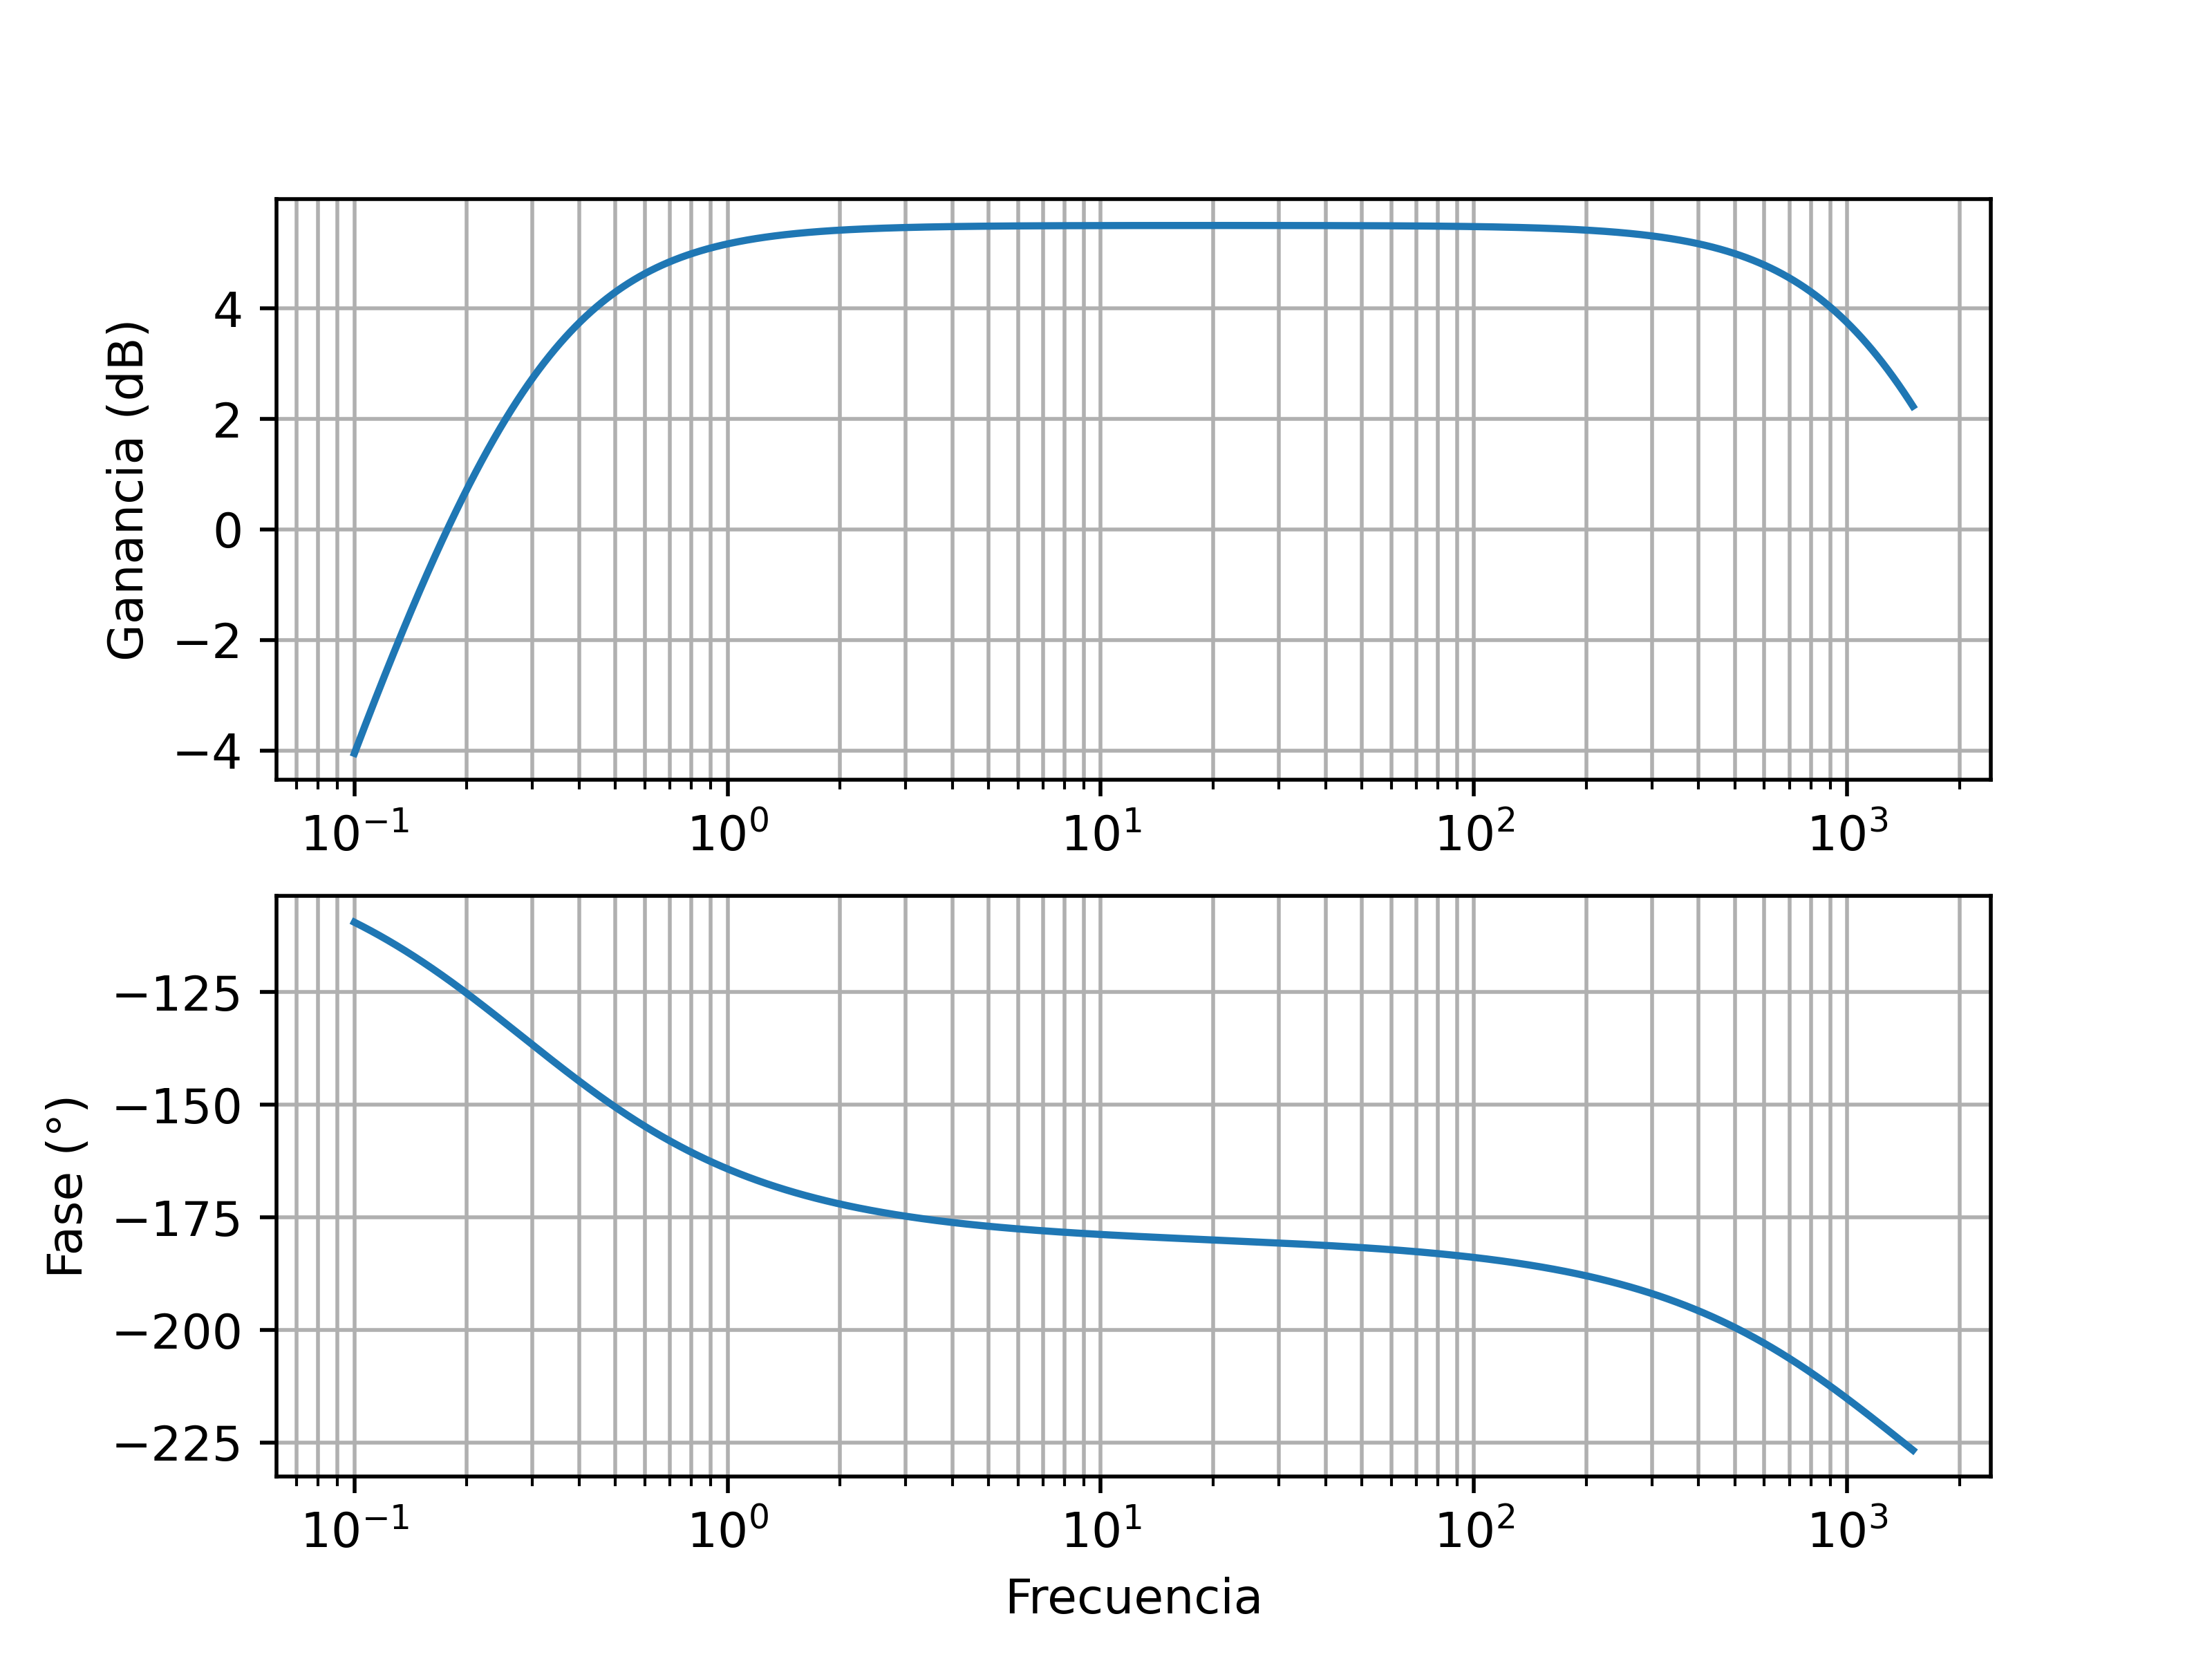
\includegraphics[width=1\textwidth]{Graficos/Bode.png}
\label{Bode}
\end{figure}
Usando el cursor vemos que para las frecuencias de interes:
\begin{table}[H]
\centering
\begin{tabular}{|c|c|c|}
\hline
& Magnitud (DB) & Fase (°) \\ \hline
\(1\,\)Hz & 5.166 & -164.42 \\ \hline
\(20\,\)Hz& 5.5 & - 180\\ \hline
\(400\,\)Hz& 5.167 & - 195.74\\ \hline
\end{tabular}
\end{table}
Donde podemos ver que cumplimos todos los requerrimientos, ganancia constante en banda pasante y \(15\)° de desfase con los extremos de la banda de interes.\\

9.
\begin{figure}[H]
\centering

\begin{subfigure}{0.45\textwidth}
    \centering
    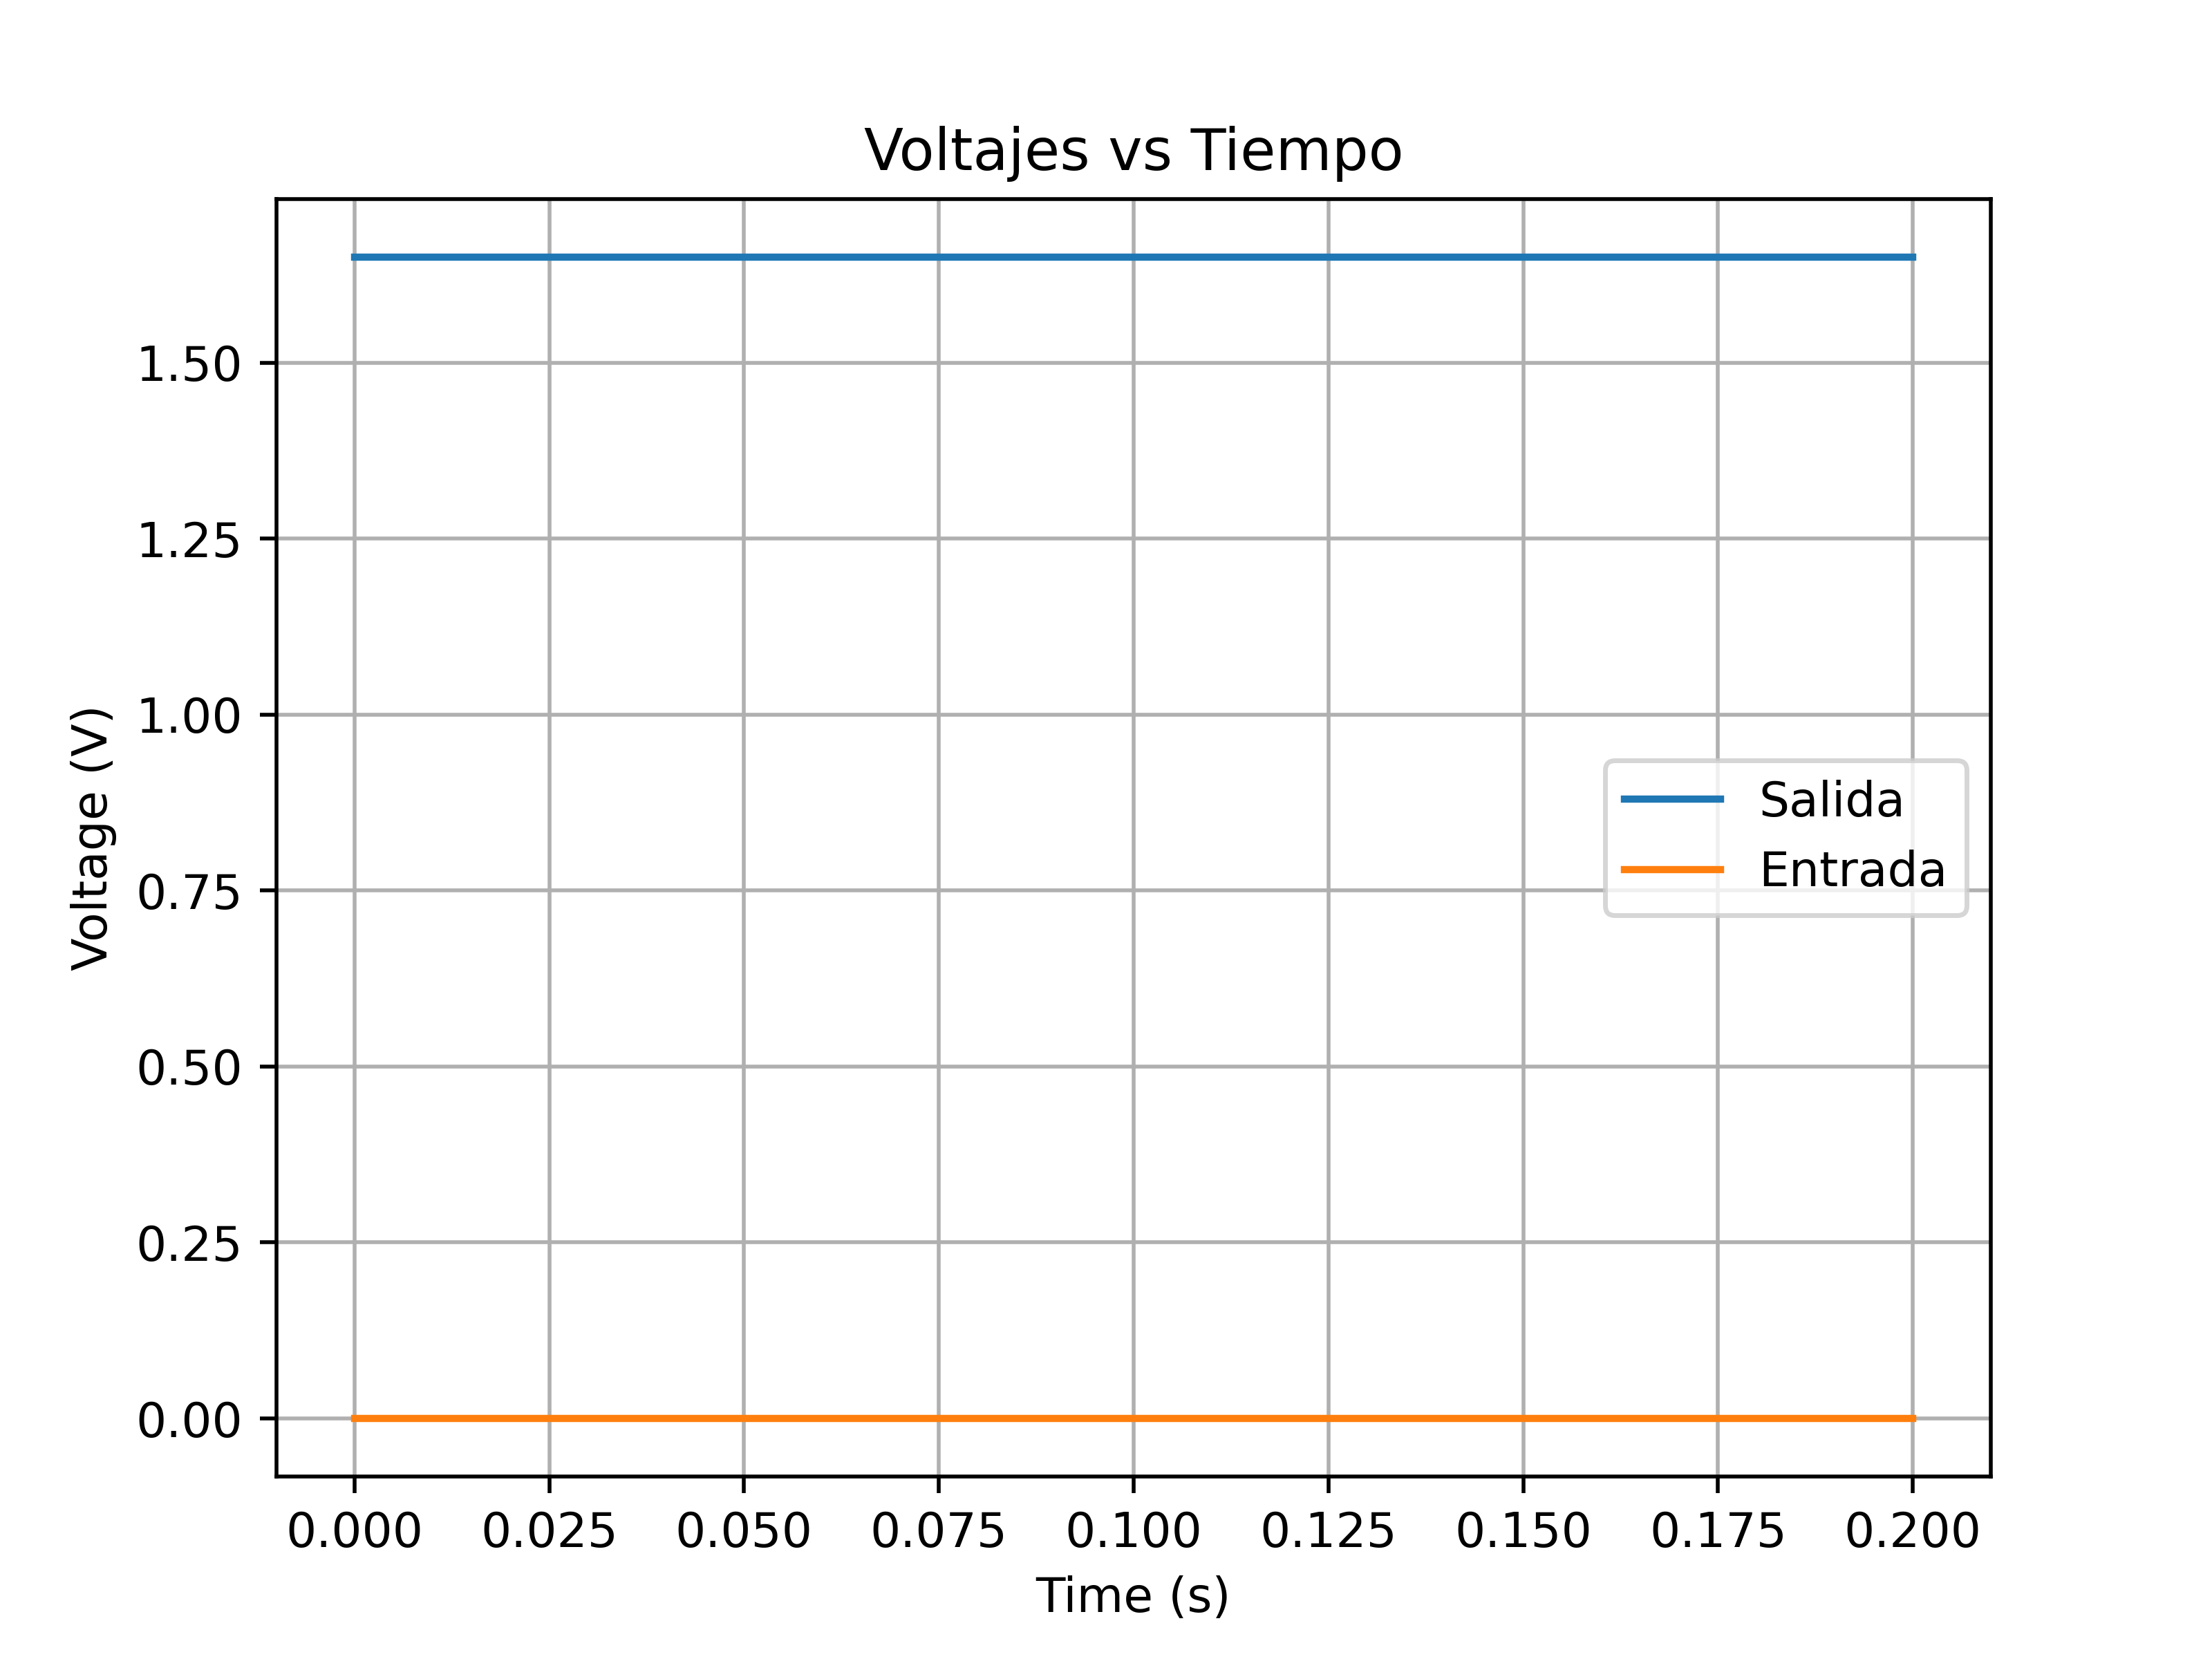
\includegraphics[width=\linewidth]{Graficos/Entrada_Nula_Graficado.png}
    \caption{}
\end{subfigure}
\hfill
\begin{subfigure}{0.45\textwidth}
    \centering
    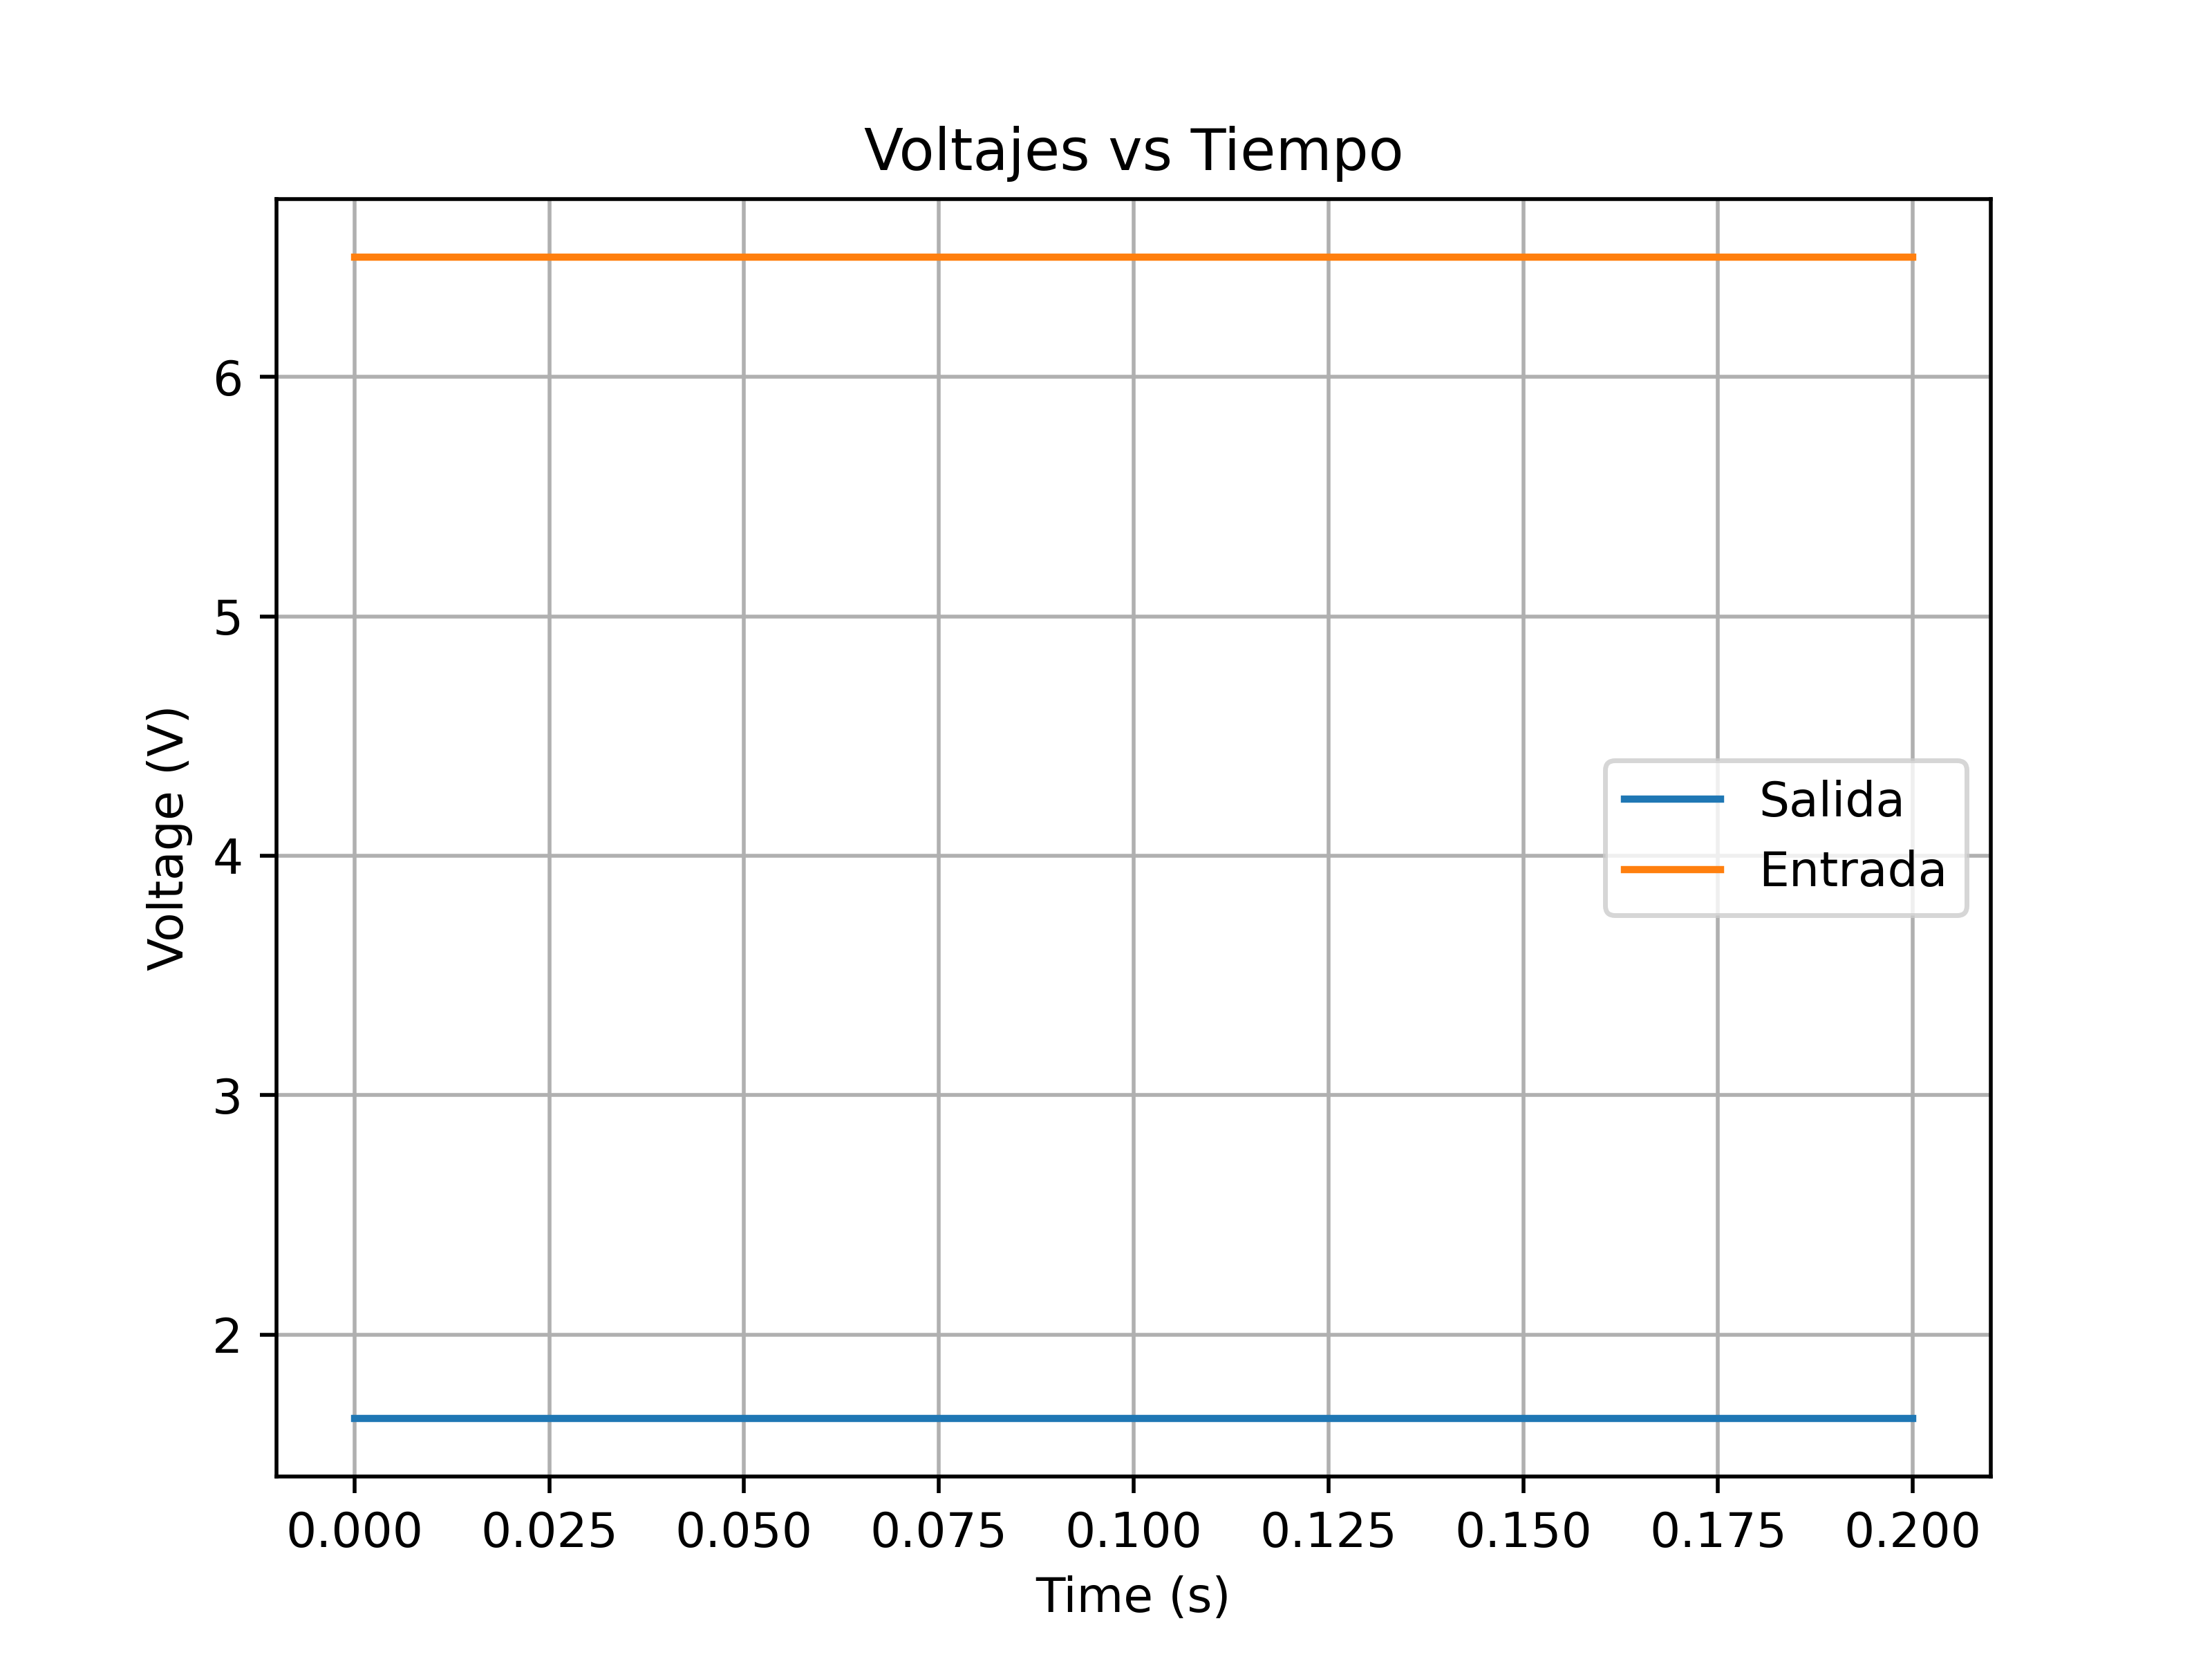
\includegraphics[width=\linewidth]{Graficos/Entrada_DC_Graficado.png}
    \caption{}
\end{subfigure}
\hfill
\begin{subfigure}{0.45\textwidth}
    \centering
    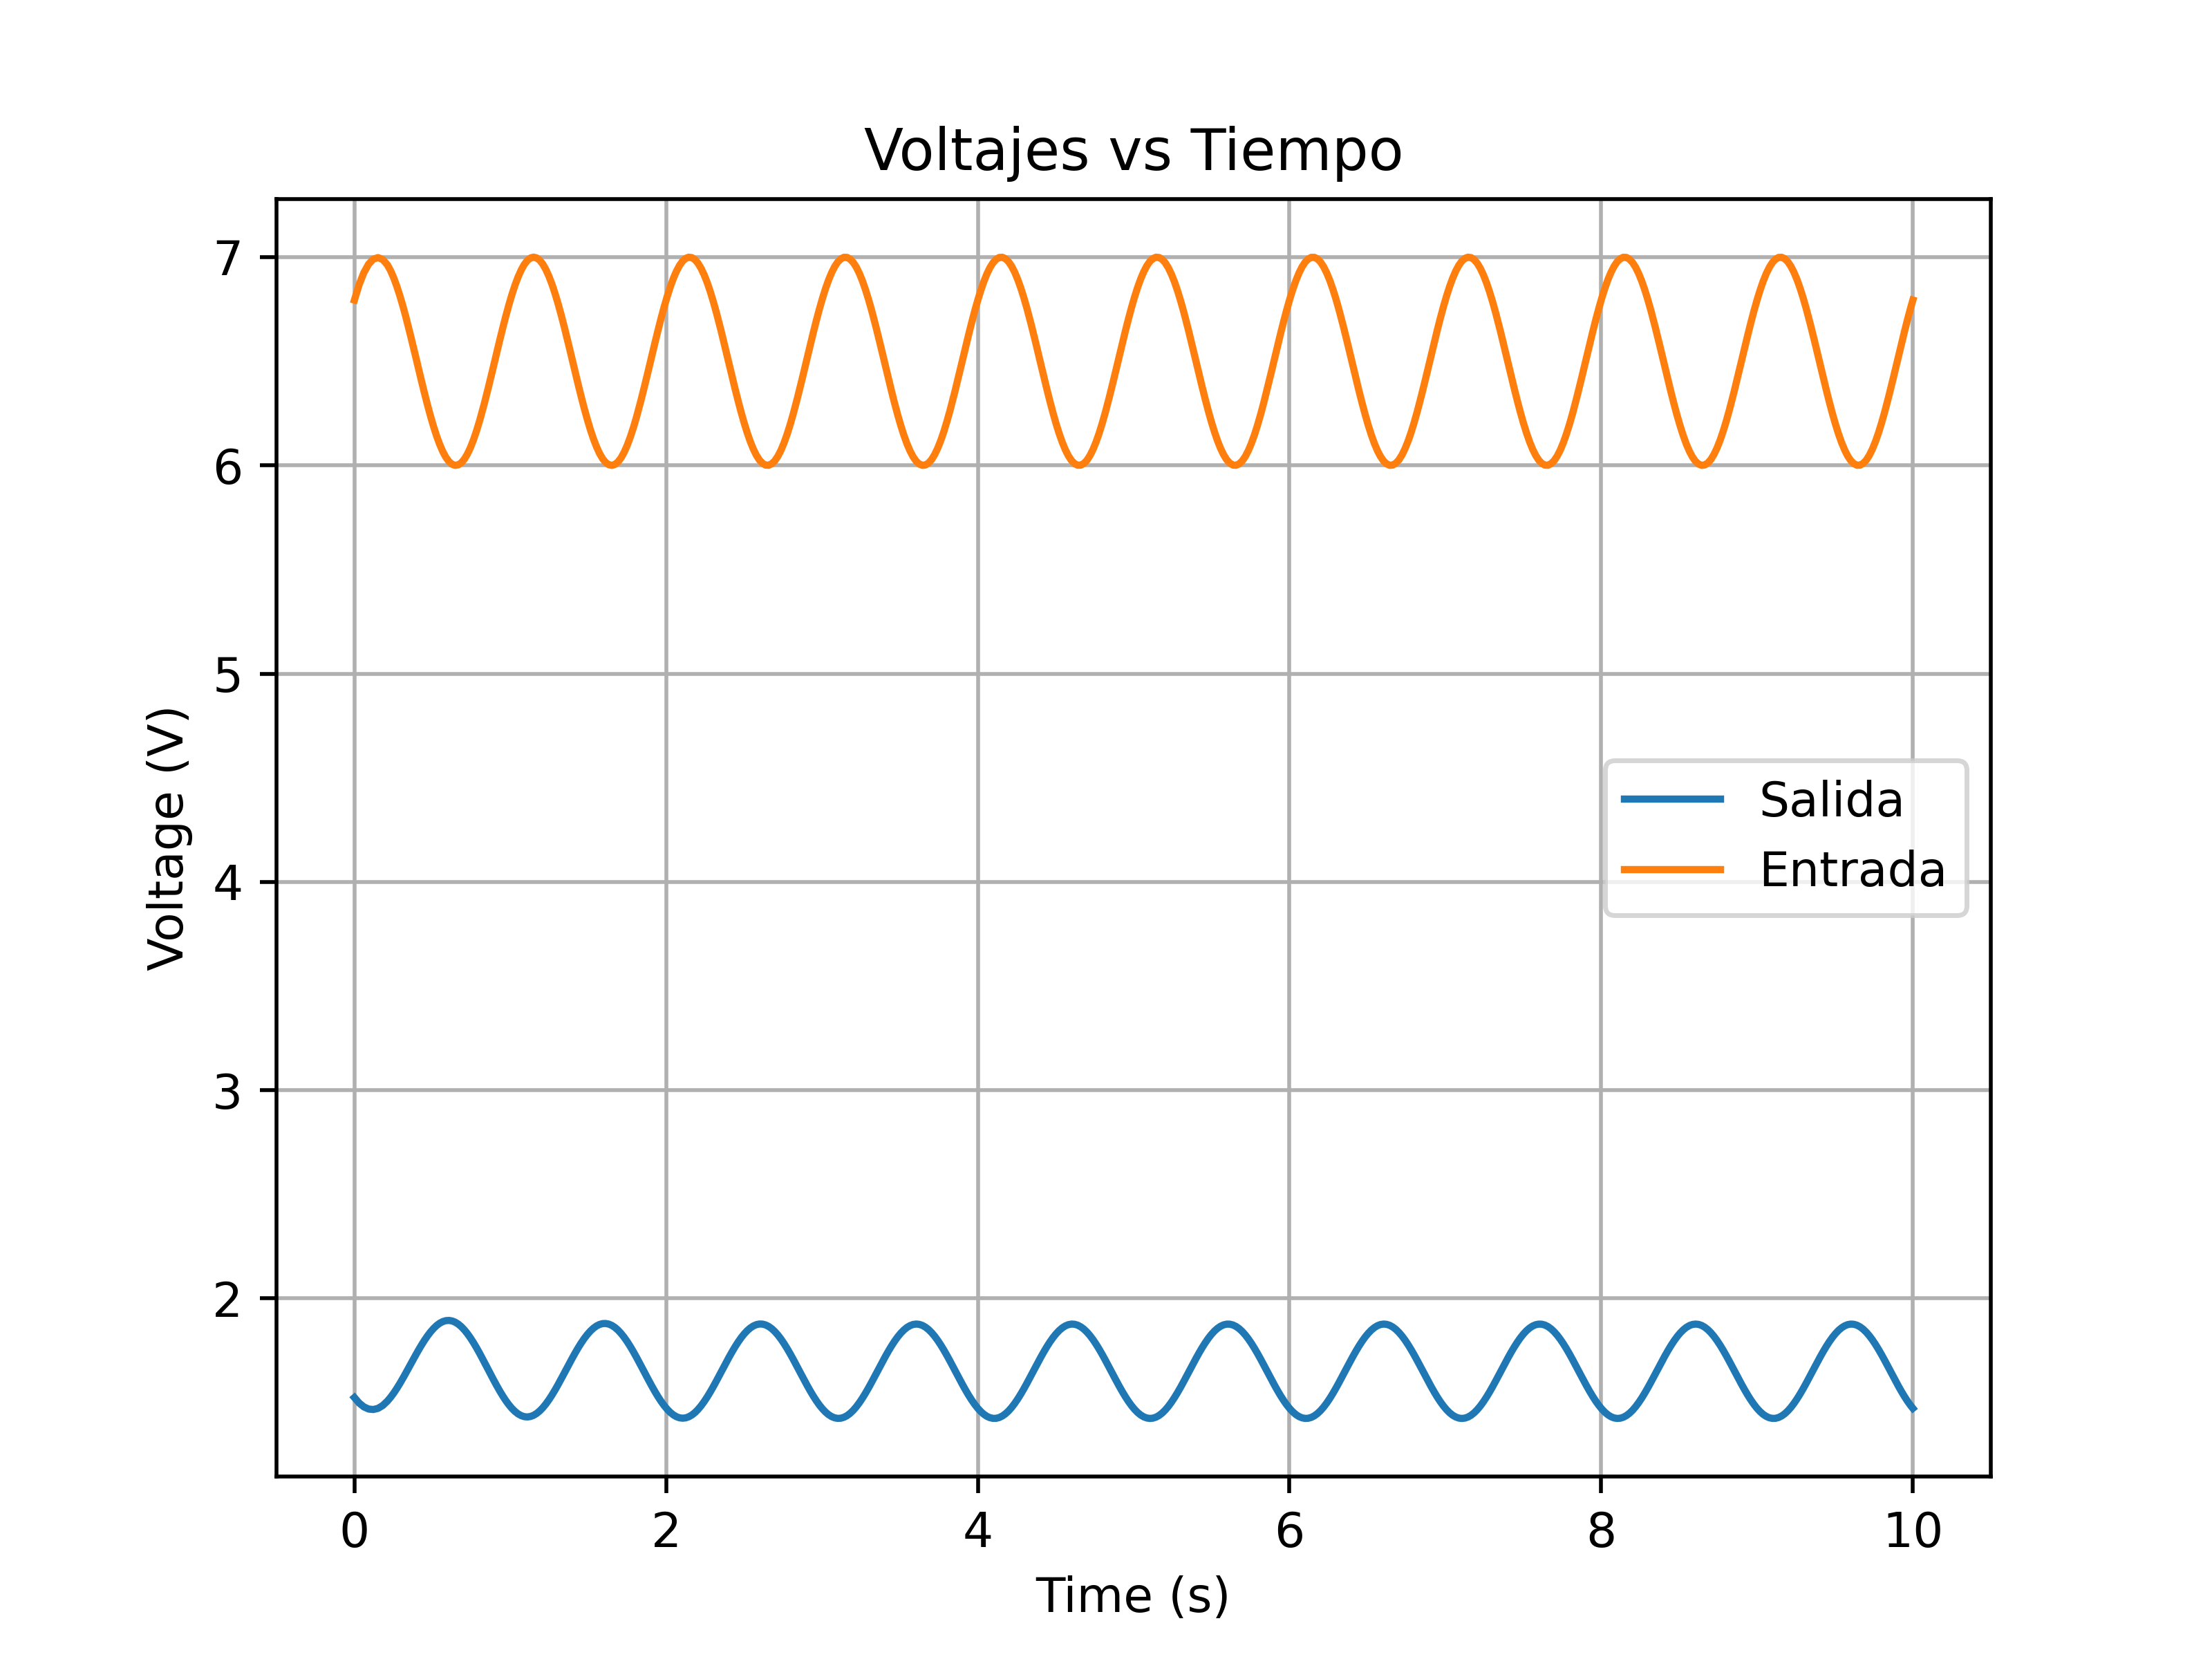
\includegraphics[width=\linewidth]{Graficos/1Hz_1pp_Graficado.png}
    \caption{}
\end{subfigure}
\hfill
\begin{subfigure}{0.45\textwidth}
    \centering
    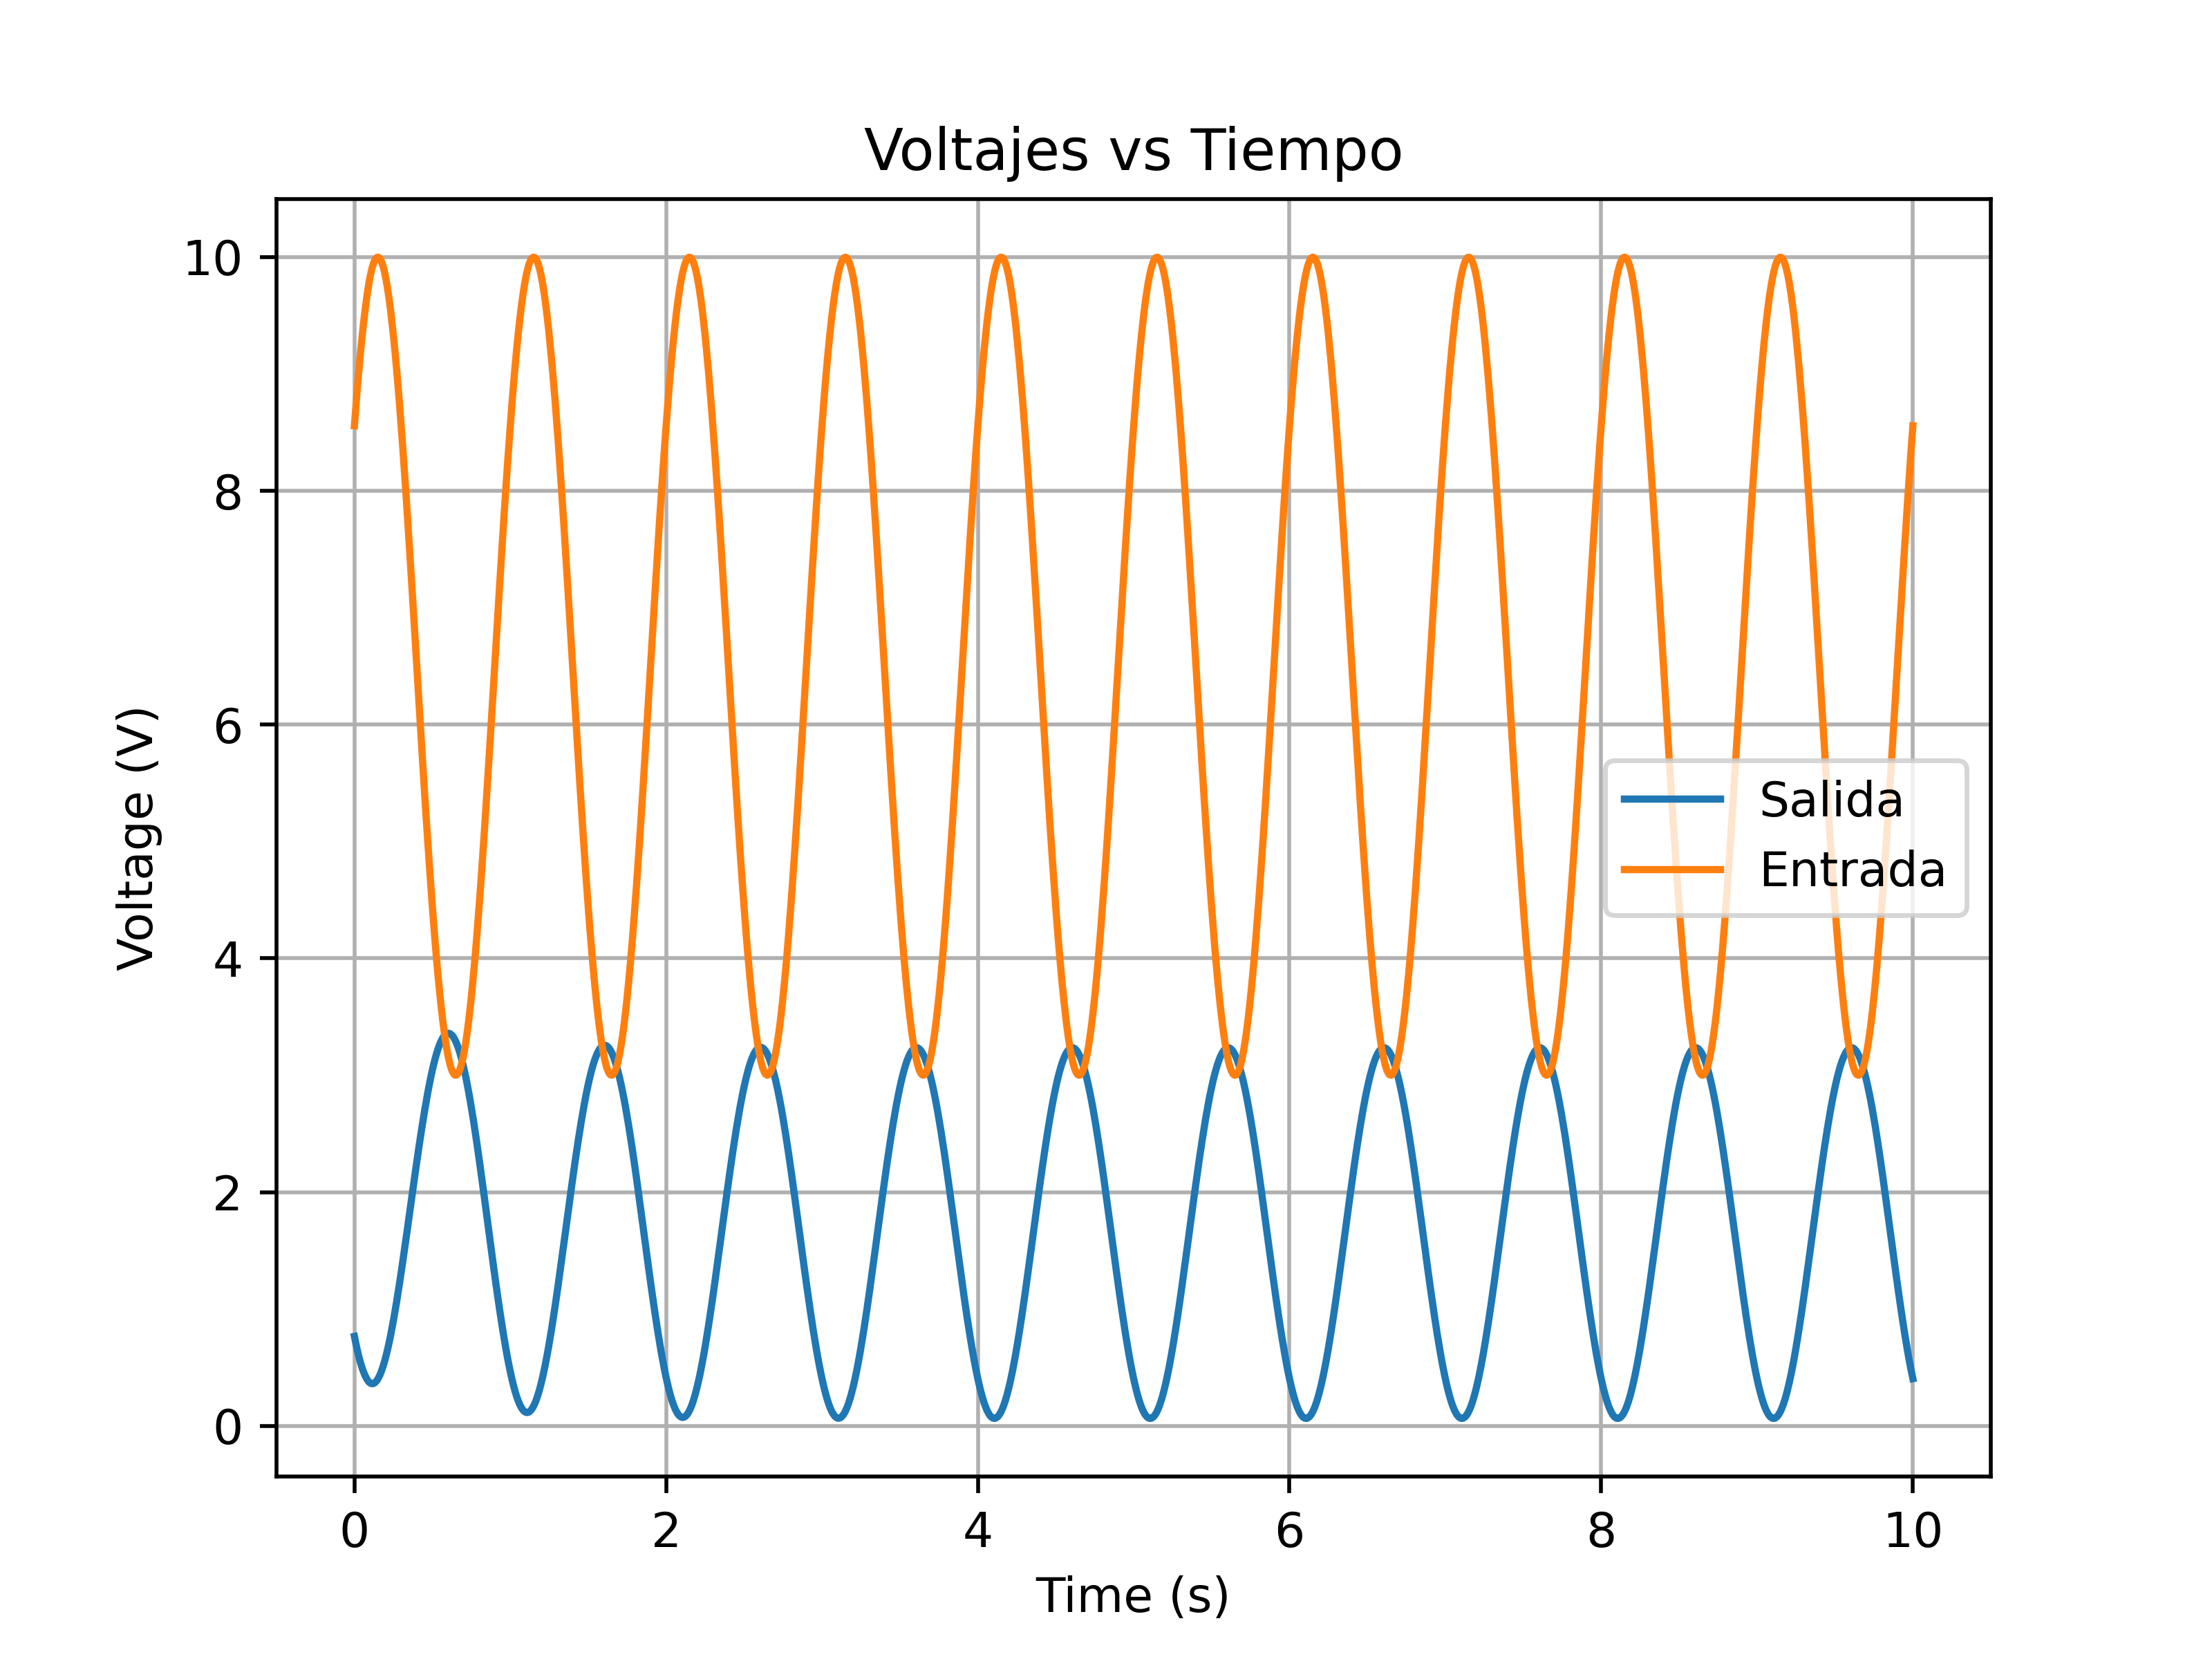
\includegraphics[width=\linewidth]{Graficos/1Hz_7pp_Graficado.png}
    \caption{}
\end{subfigure}
\hfill
\begin{subfigure}{0.45\textwidth}
    \centering
    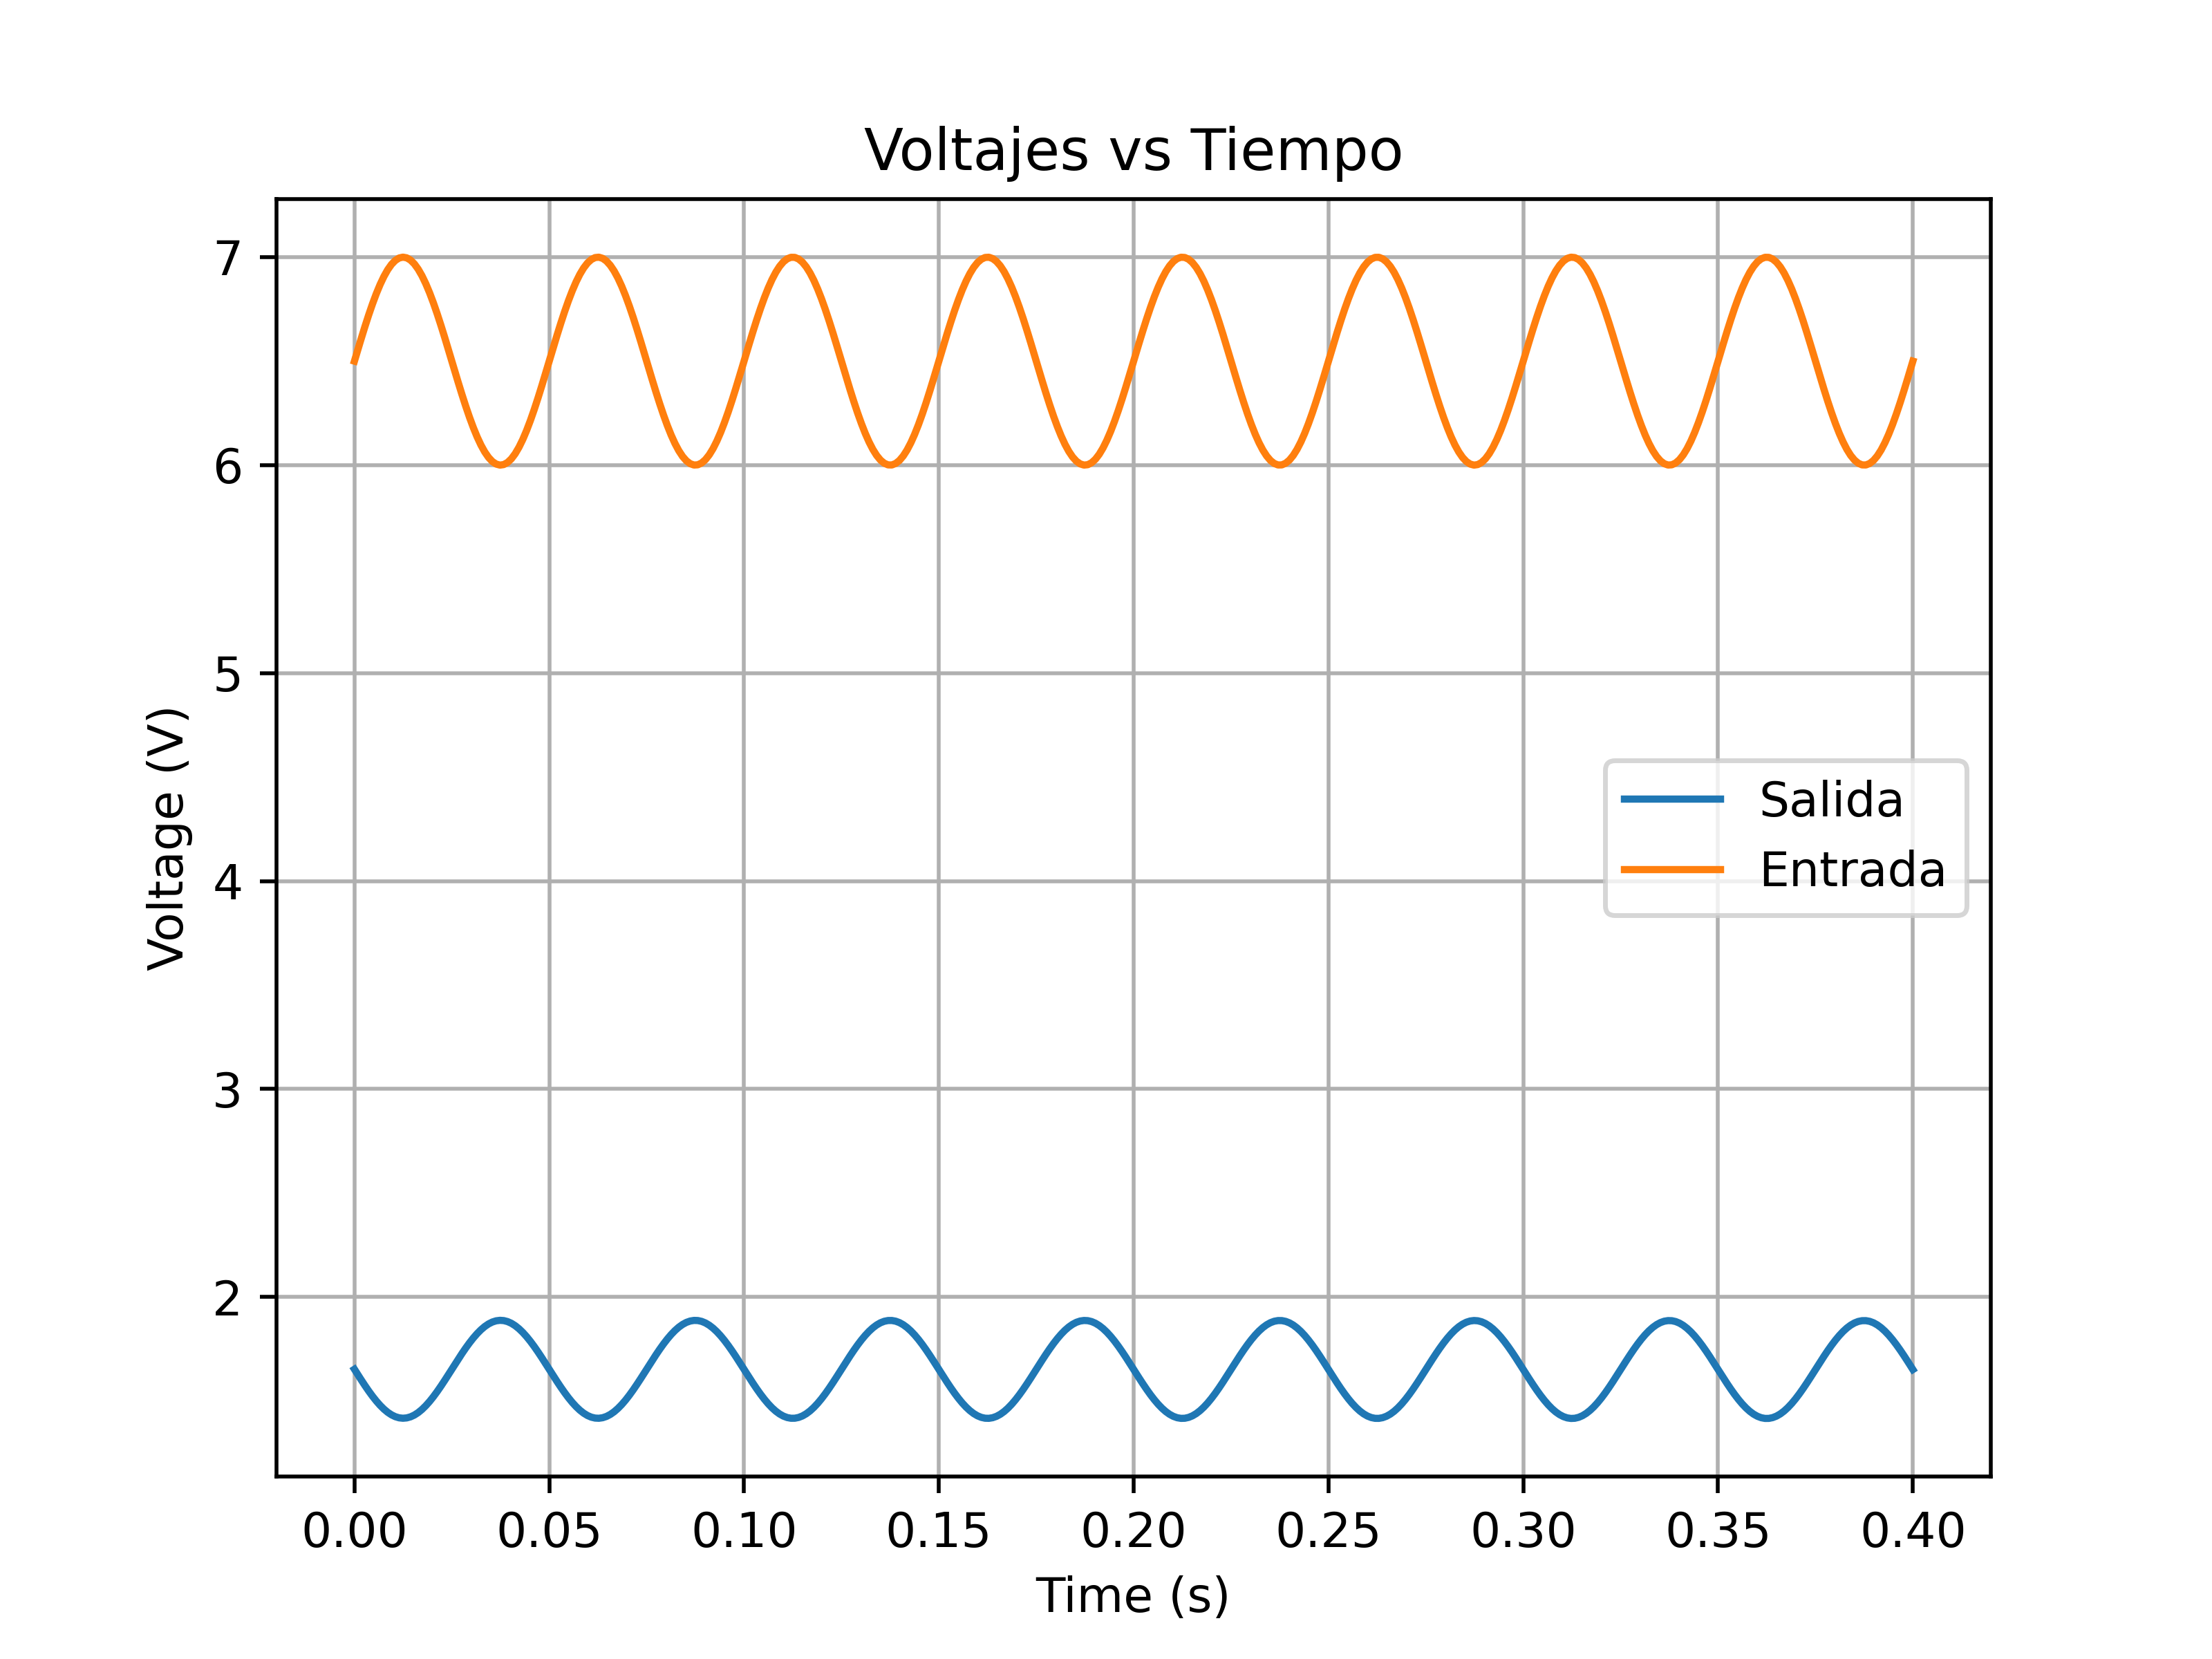
\includegraphics[width=\linewidth]{Graficos/20Hz_1pp_Graficado.png}
    \caption{}
\end{subfigure}
\hfill
\begin{subfigure}{0.45\textwidth}
    \centering
    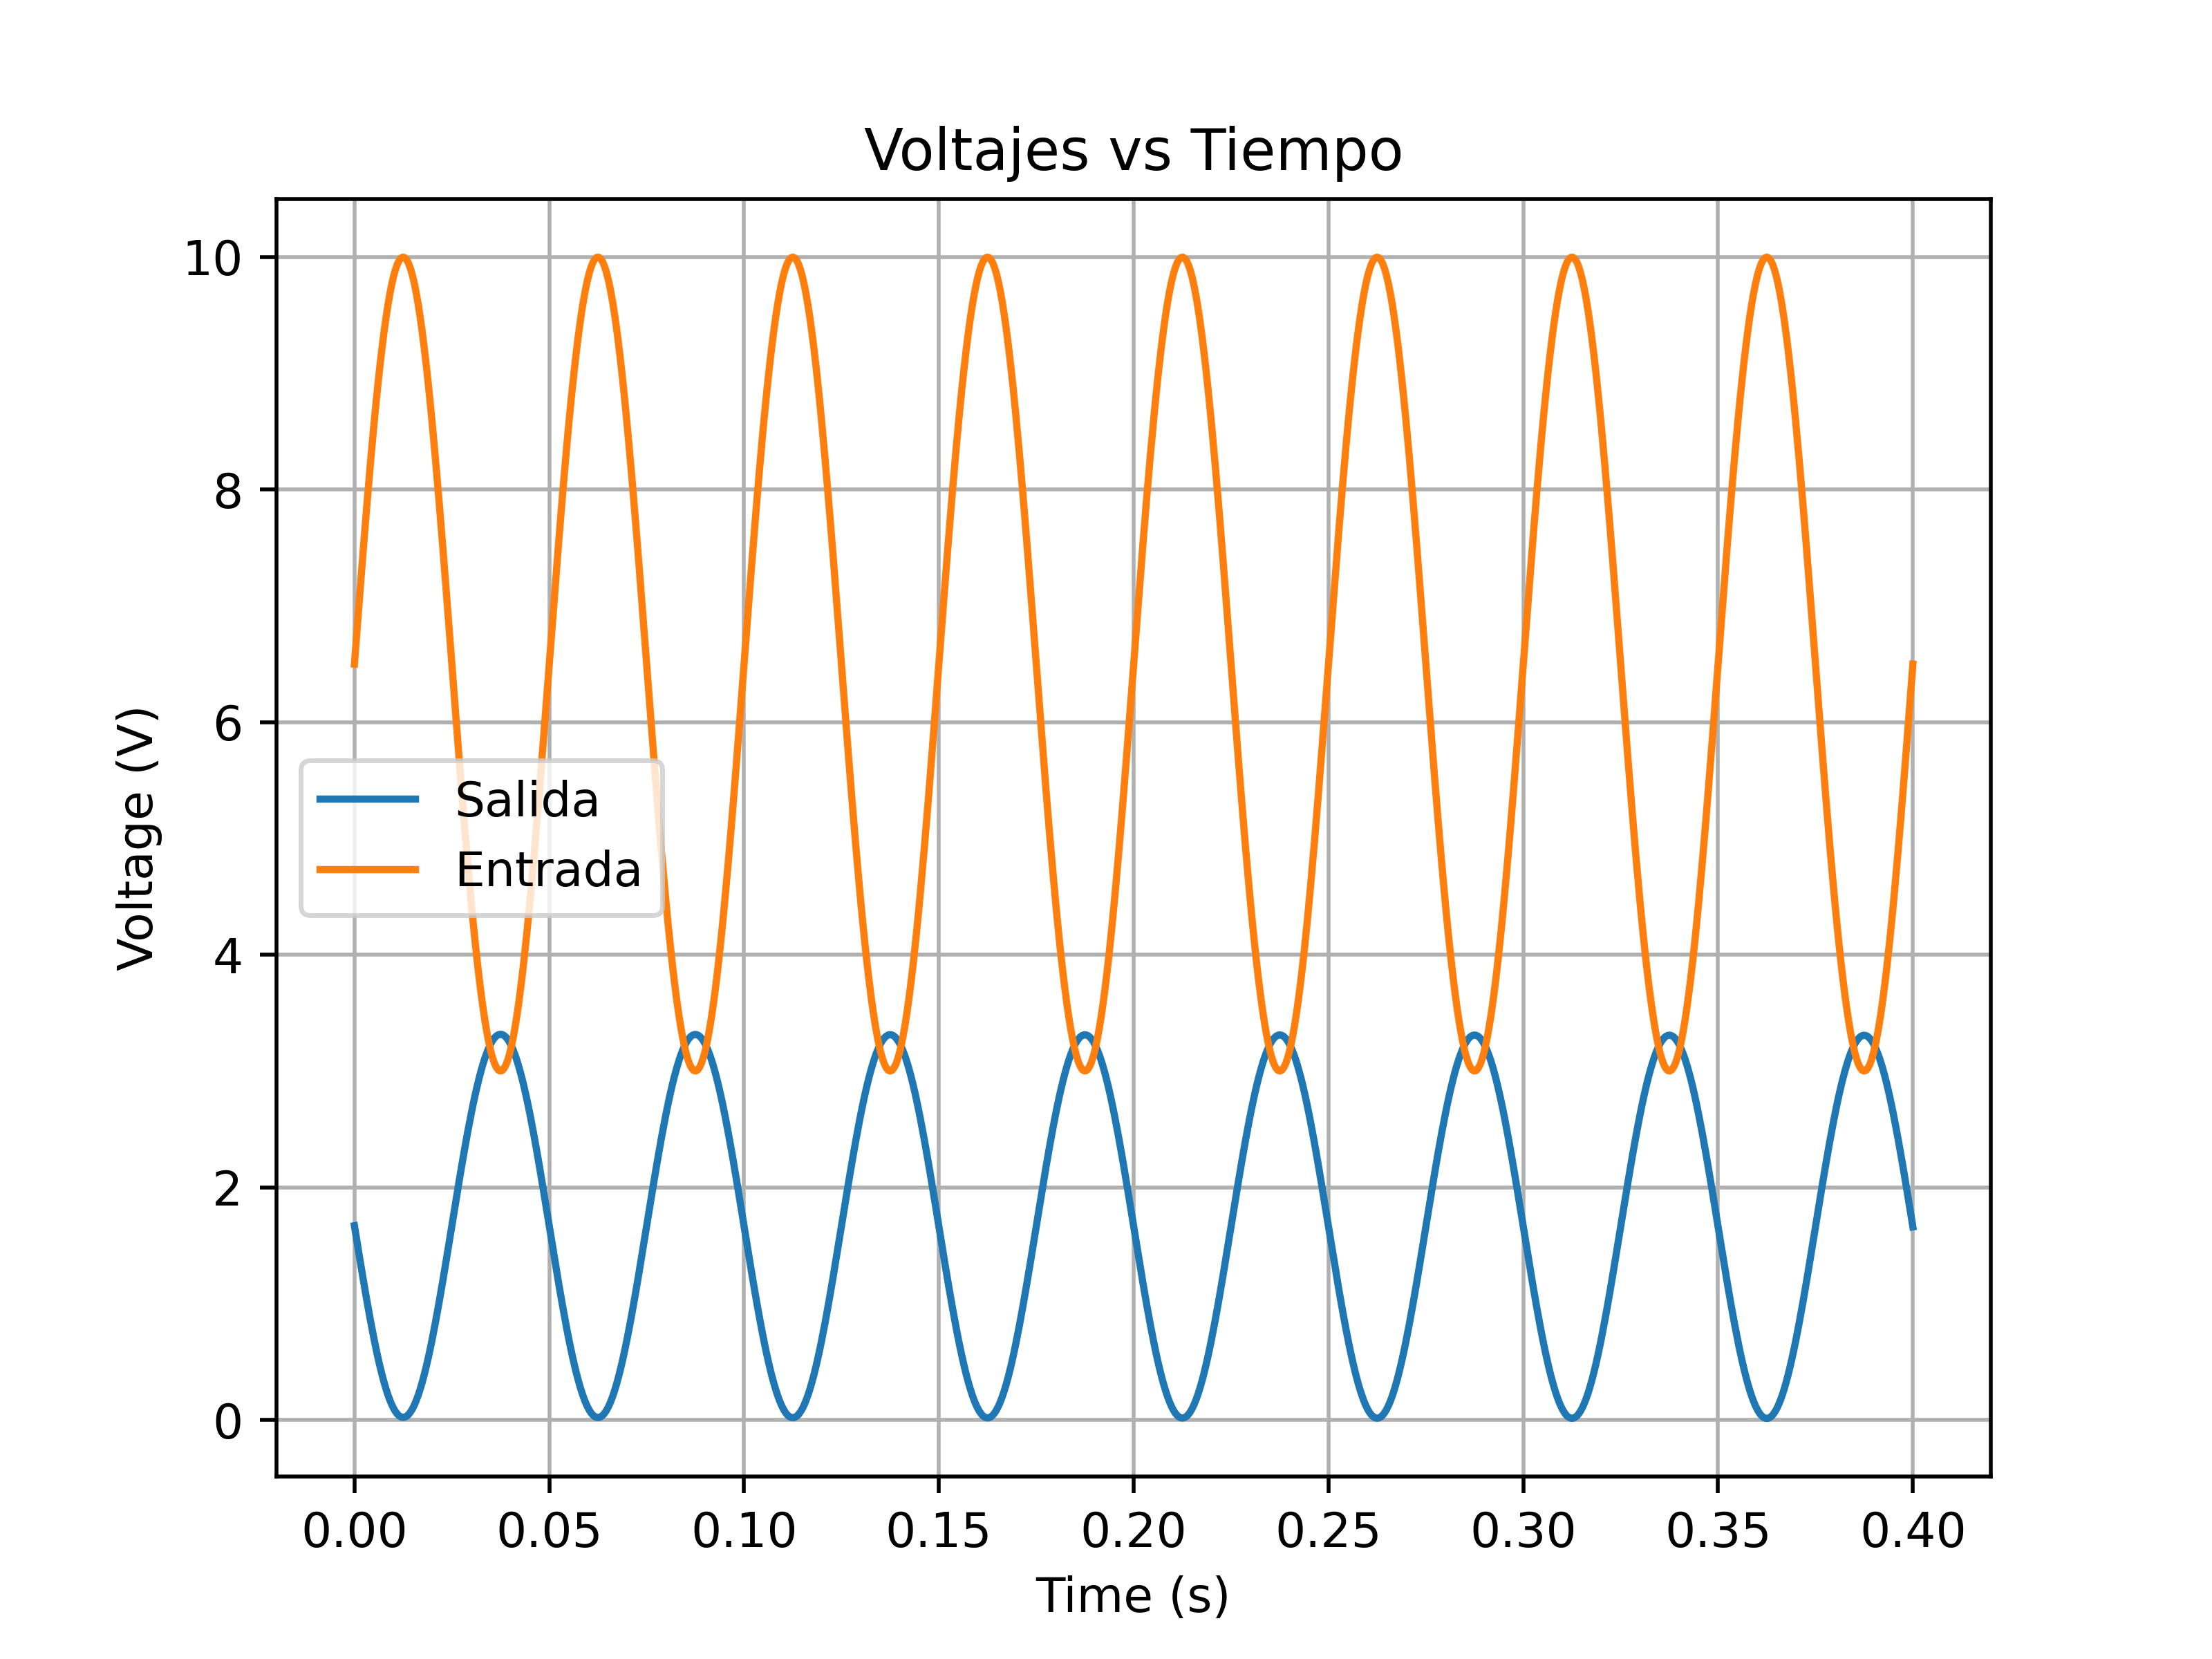
\includegraphics[width=\linewidth]{Graficos/20Hz_7pp_Graficado.png}
    \caption{}
\end{subfigure}
\hfill
\begin{subfigure}{0.45\textwidth}
    \centering
    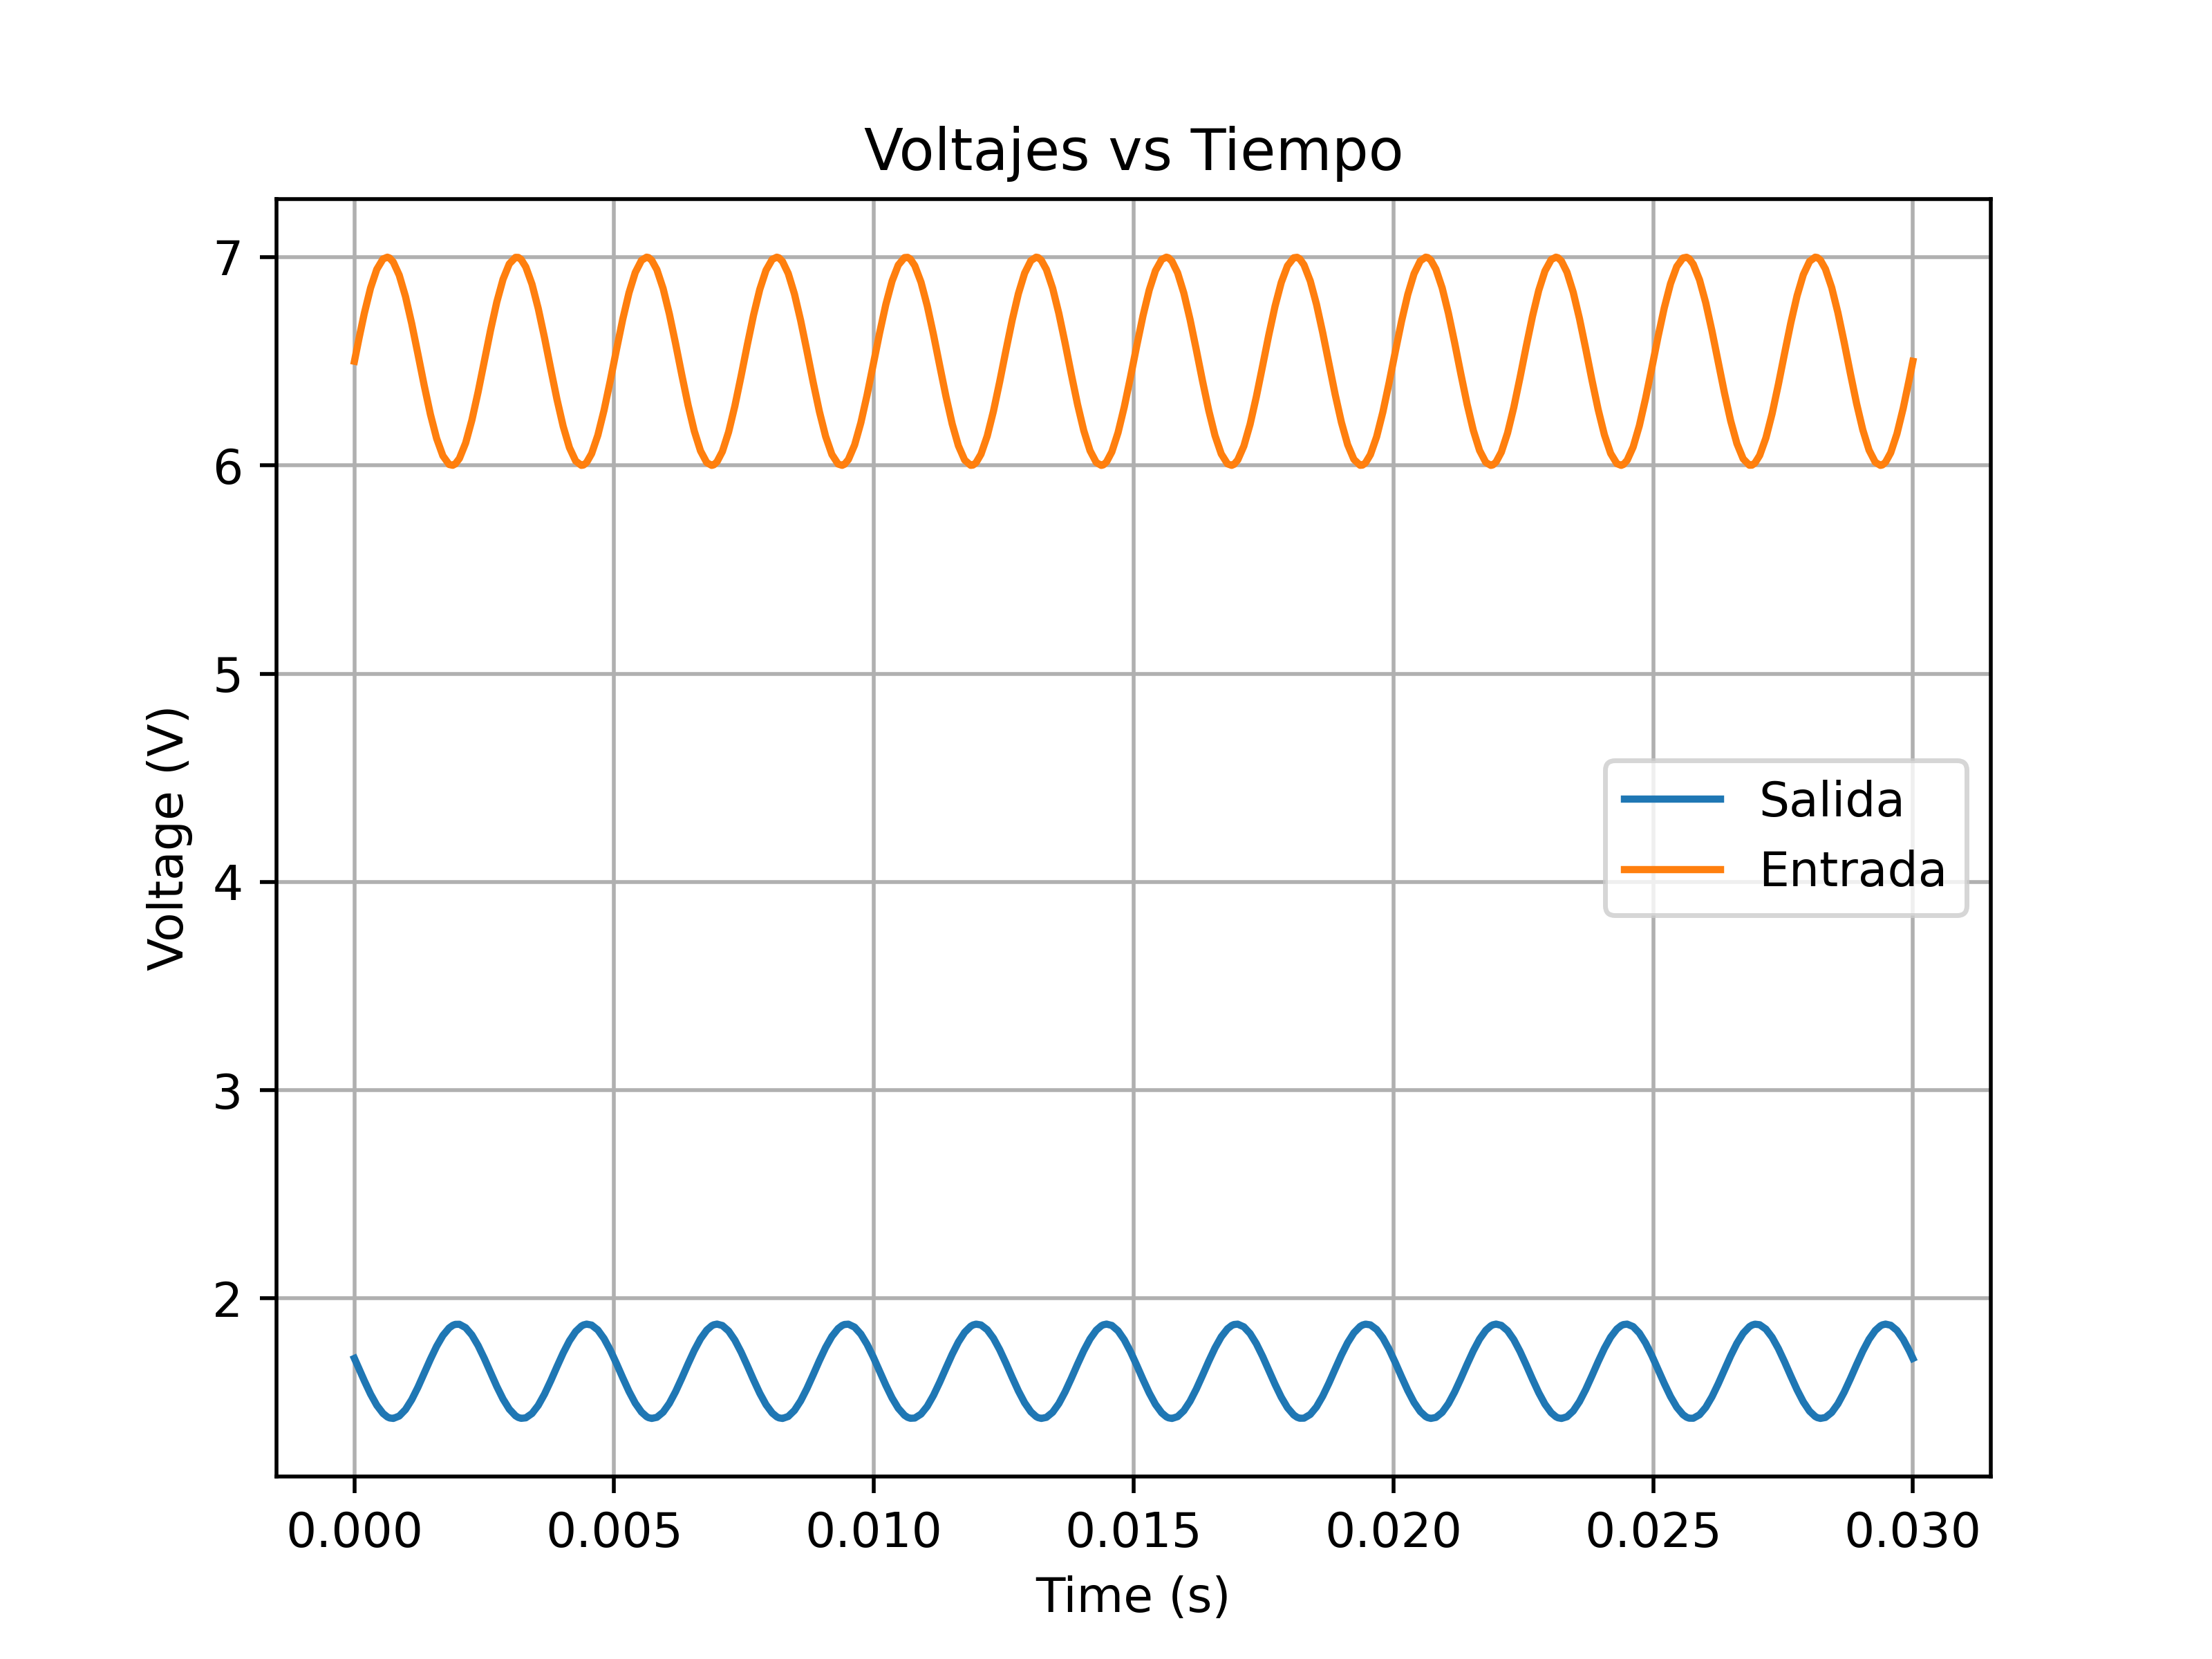
\includegraphics[width=\linewidth]{Graficos/400Hz_1pp_Graficado.png}
    \caption{}
\end{subfigure}
\hfill
\begin{subfigure}{0.45\textwidth}
    \centering
    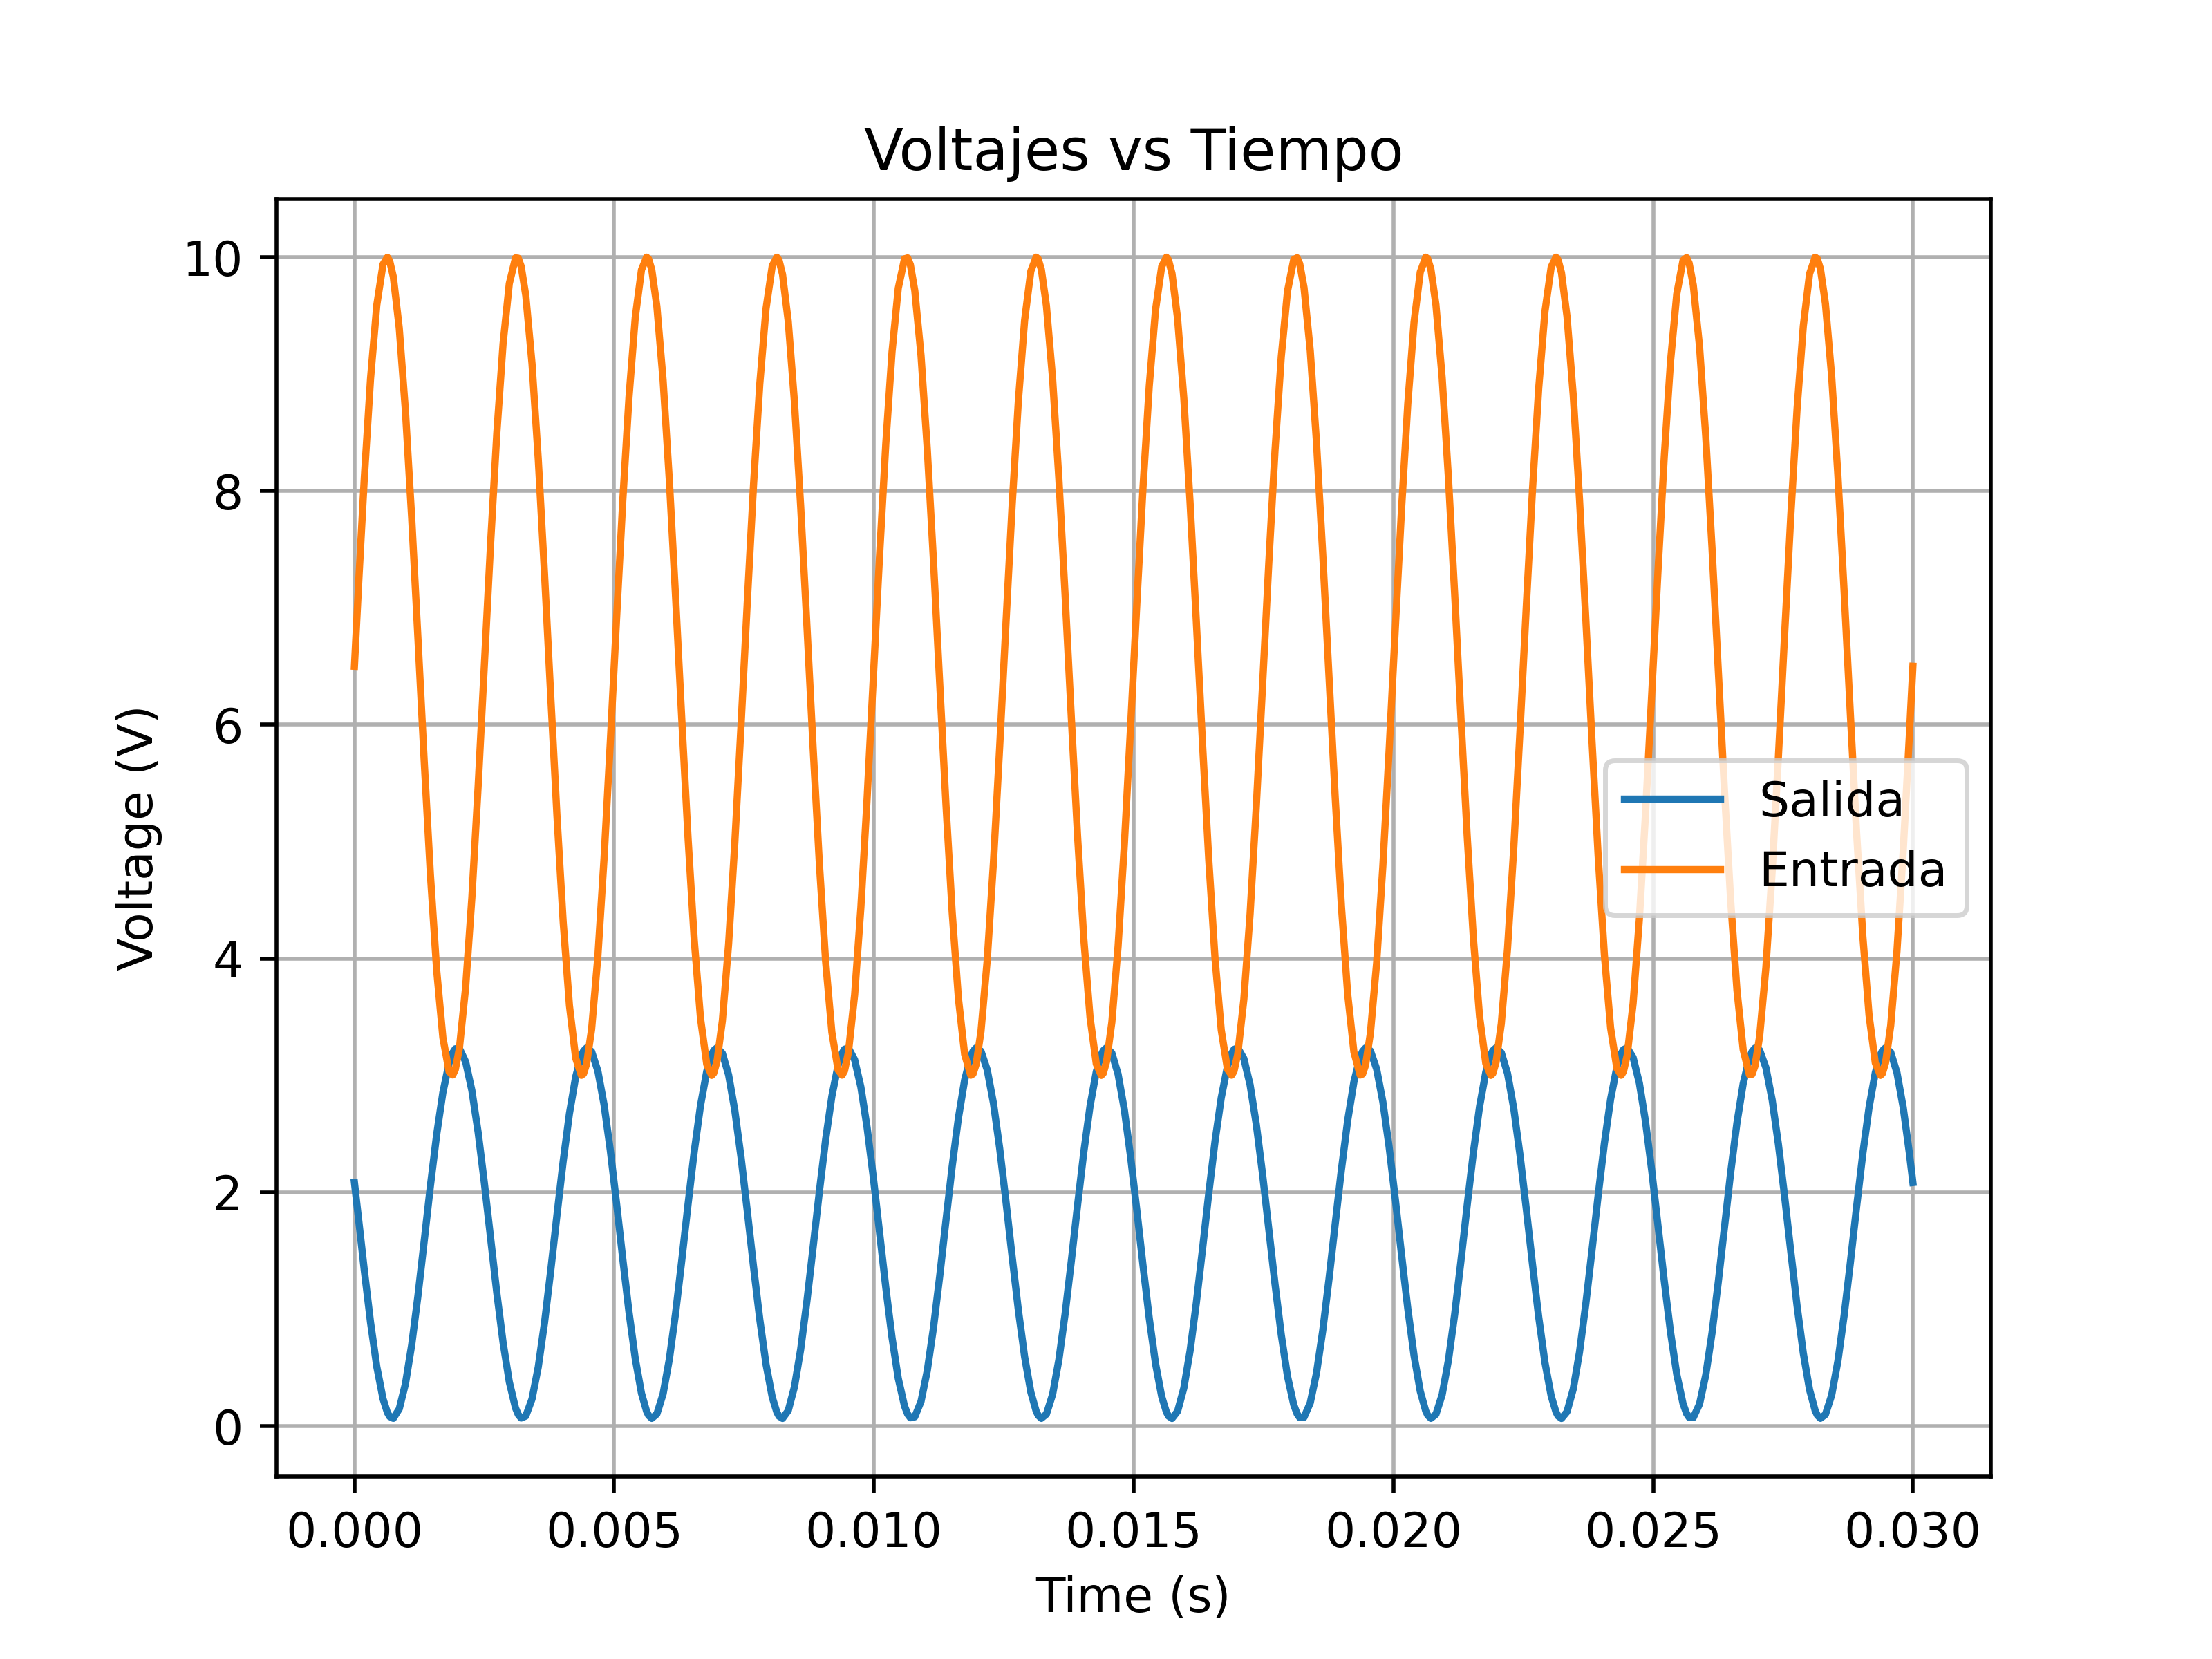
\includegraphics[width=\linewidth]{Graficos/400Hz_7pp_Graficado.png}
    \caption{}
\end{subfigure}
\end{figure}
i) \begin{table}[H]
\centering
\begin{tabular}{|c|c|}
\hline
Pregunta & Desfase (°)  \\ \hline
\(c)\,\) & - 164.12 \\ \hline
\(e)\,\)& -180.43 \\ \hline
\(g)\,\)& -195.84\\ \hline
\end{tabular}
\end{table}



\noindent\rule{\textwidth}{0.4pt}

\subsection{ESP32}

1. Investigue sobre las protecciones (si aplica) y los rangos de voltaje admisibles del ADC integrado en el microcontrolador.
\subsection*{\small\textbf{Respuesta:}}
El ADC integrado en el ESP32 admite voltajes de entrada entre 0V y 3,3V, con protecciones internas mediante diodos de sujeción (clamping diodes) en los GPIOs. Para voltajes mayores al de referencia (Vref $\approx$ 1,1V), se emplea atenuación configurada por software.

En realidad, el ADC del ESP32 no admite directamente voltajes entre 0V y 3,3V a la entrada, sino que admite voltajes entre 0V y 1,1V (o un voltaje cercano, puesto que depende del ESP32 utilizado). Sin embargo, el propio ADC puede ser configurado para atenuar la señal de entrada antes de ser convertida, por lo que, en ese caso, dependiendo de la atenuación, el ADC puede admitir voltajes de entradas mayores, hasta llegar a los 3,3V.

{\small\textbf{Modo de atenuación:}}
\begin{itemize}
    \item 0 dB: rango de entrada 0-1,1V ó 0-Vref (Sin atenuación)
    \item 2,5 dB: rango de entrada 0-1,5V
    \item 6 dB: rango de entrada 0-2,2V
    \item 11 dB: rango de entrada 0-3,3V (Máxima atenuación y covertura)
\end{itemize}
Notese que en el modo de ``\textit{sin atenuación}'' se coloca 0-Vref, puesto que usualmente Vref es un valor cercano a 1,1V, pero dependiendo del ESP32 este valor podría variar levemente.

Por otro lado, al inicio se mencionó que el ADC presenta protecciones internas mediante diodos de sujeción; estos, más especificamente, limitan sobretensiones de voltaje desviando la corriente hacia la alimentación o tierra. Sin embargo, aunque estos diodos protegen contra picos de voltaje breves, {\small\textbf{no sustituyen un circuito de protección externo.}} Por esto, es bueno usar divisores de voltaje, resistencias en serie u otros circuitos que protejan al ADC si se cree que este podría ser sometido a voltajes de entrada mayores a 3,3V o a un voltaje de entrada mayor al que resiste el modo de atenuación configurado.

\newpage

2. Investigue cuáles son las ventajas y desventajas de los protocolos de comunicación serial y paralelo. ¿Qué pines pueden ser utilizados para los protocolos serial?

\subsection*{\small\textbf{Respuesta:}}

{\small\textbf{Comunicación Paralela}}

Se envían múltiples bits de datos de forma simultánea a través de varios canales al mismo tiempo.

{\footnotesize\textbf{Ventajas:}}

\begin{itemize}
    \item Velocidad en distancias cortas: Al enviar muchos bits a la vez, el volumen de datos transferido por ciclo de reloj es muy alto.
    \item Simplicidad lógica: No requiere procesos complejos de ``empaquetado'' de datos; los datos se envían tal como están en el bus del sistema.
\end{itemize}

{\footnotesize\textbf{Desventajas:}}

\begin{itemize}
    \item Crosstalk (Interferencia): Al haber muchos cables juntos, las señales eléctricas de uno pueden interferir en el otro, corrompiendo los datos.
    \item Skew (Desincronización): En cables largos, los bits pueden llegar en momentos ligeramente distintos debido a pequeñas variaciones físicas, lo que causa errores de lectura.
    \item Costo y tamaño: Requiere cables más gruesos y conectores más grandes.
\end{itemize}

{\small\textbf{Comunicación Serial}}

Se envían los datos bit a bit, a través de un solo canal o par de hilos.

{\footnotesize\textbf{Ventajas}}

\begin{itemize}
    \item Integridad en largas distancias: Al no haber cables adyacentes transmitiendo al mismo tiempo, se eliminan el \textit{crosswalk} y el \textit{skew}.
    \item Menos cables, menos espacio: Los conectores son pequeños, lo que facilita la ventilación y el diseño de dispositivos compactos.
    \item Frecuencias más altas: Gracias a la falta de interferencias, los protocolos seriales modernos pueden funcionar a velocidades de reloj altísimas, superando en la práctica a los paralelos.
\end{itemize}

{\footnotesize\textbf{Desventajas}}

\begin{itemize}
    \item Complejidad de procesamiento: Requiere circuitería adicional para convertir los datos de paralelo a serial y viceversa.
    \item Latencia de protocolo: A veces el software y el hardware necesitan coordinarse más veces para asegurar que los bits lleguen en el orden correcto.
\end{itemize}

Para efectos de nuestro trabajo en el ESP32, la comunicación serial es más práctica por su {\small\textbf{flexibilidad y menor consumo de pines.}}

Gracias al GPIO Matrix, el ESP32 permite asignar casi cualquier pin a funciones seriales, sin embargo, algunos protocolos seriales tienen asignaciones de pines por defecto (ej. GPIO1/3 para UART, GPIO21/22 para $\text{I}^{2}$C).

\noindent\rule{\textwidth}{0.4pt}

\subsection{FPGA}

1. Realice un diagrama de bloques, explicitando las entradas y salidas, así como el tamaño de los buses de datos utilizados. Explique que realiza cada bloque.\\

\textbf{Respuesta:}\\

El diagrama de bloques realizado para esta experiencia es el siguiente:

\begin{figure}[H]
    \centering
    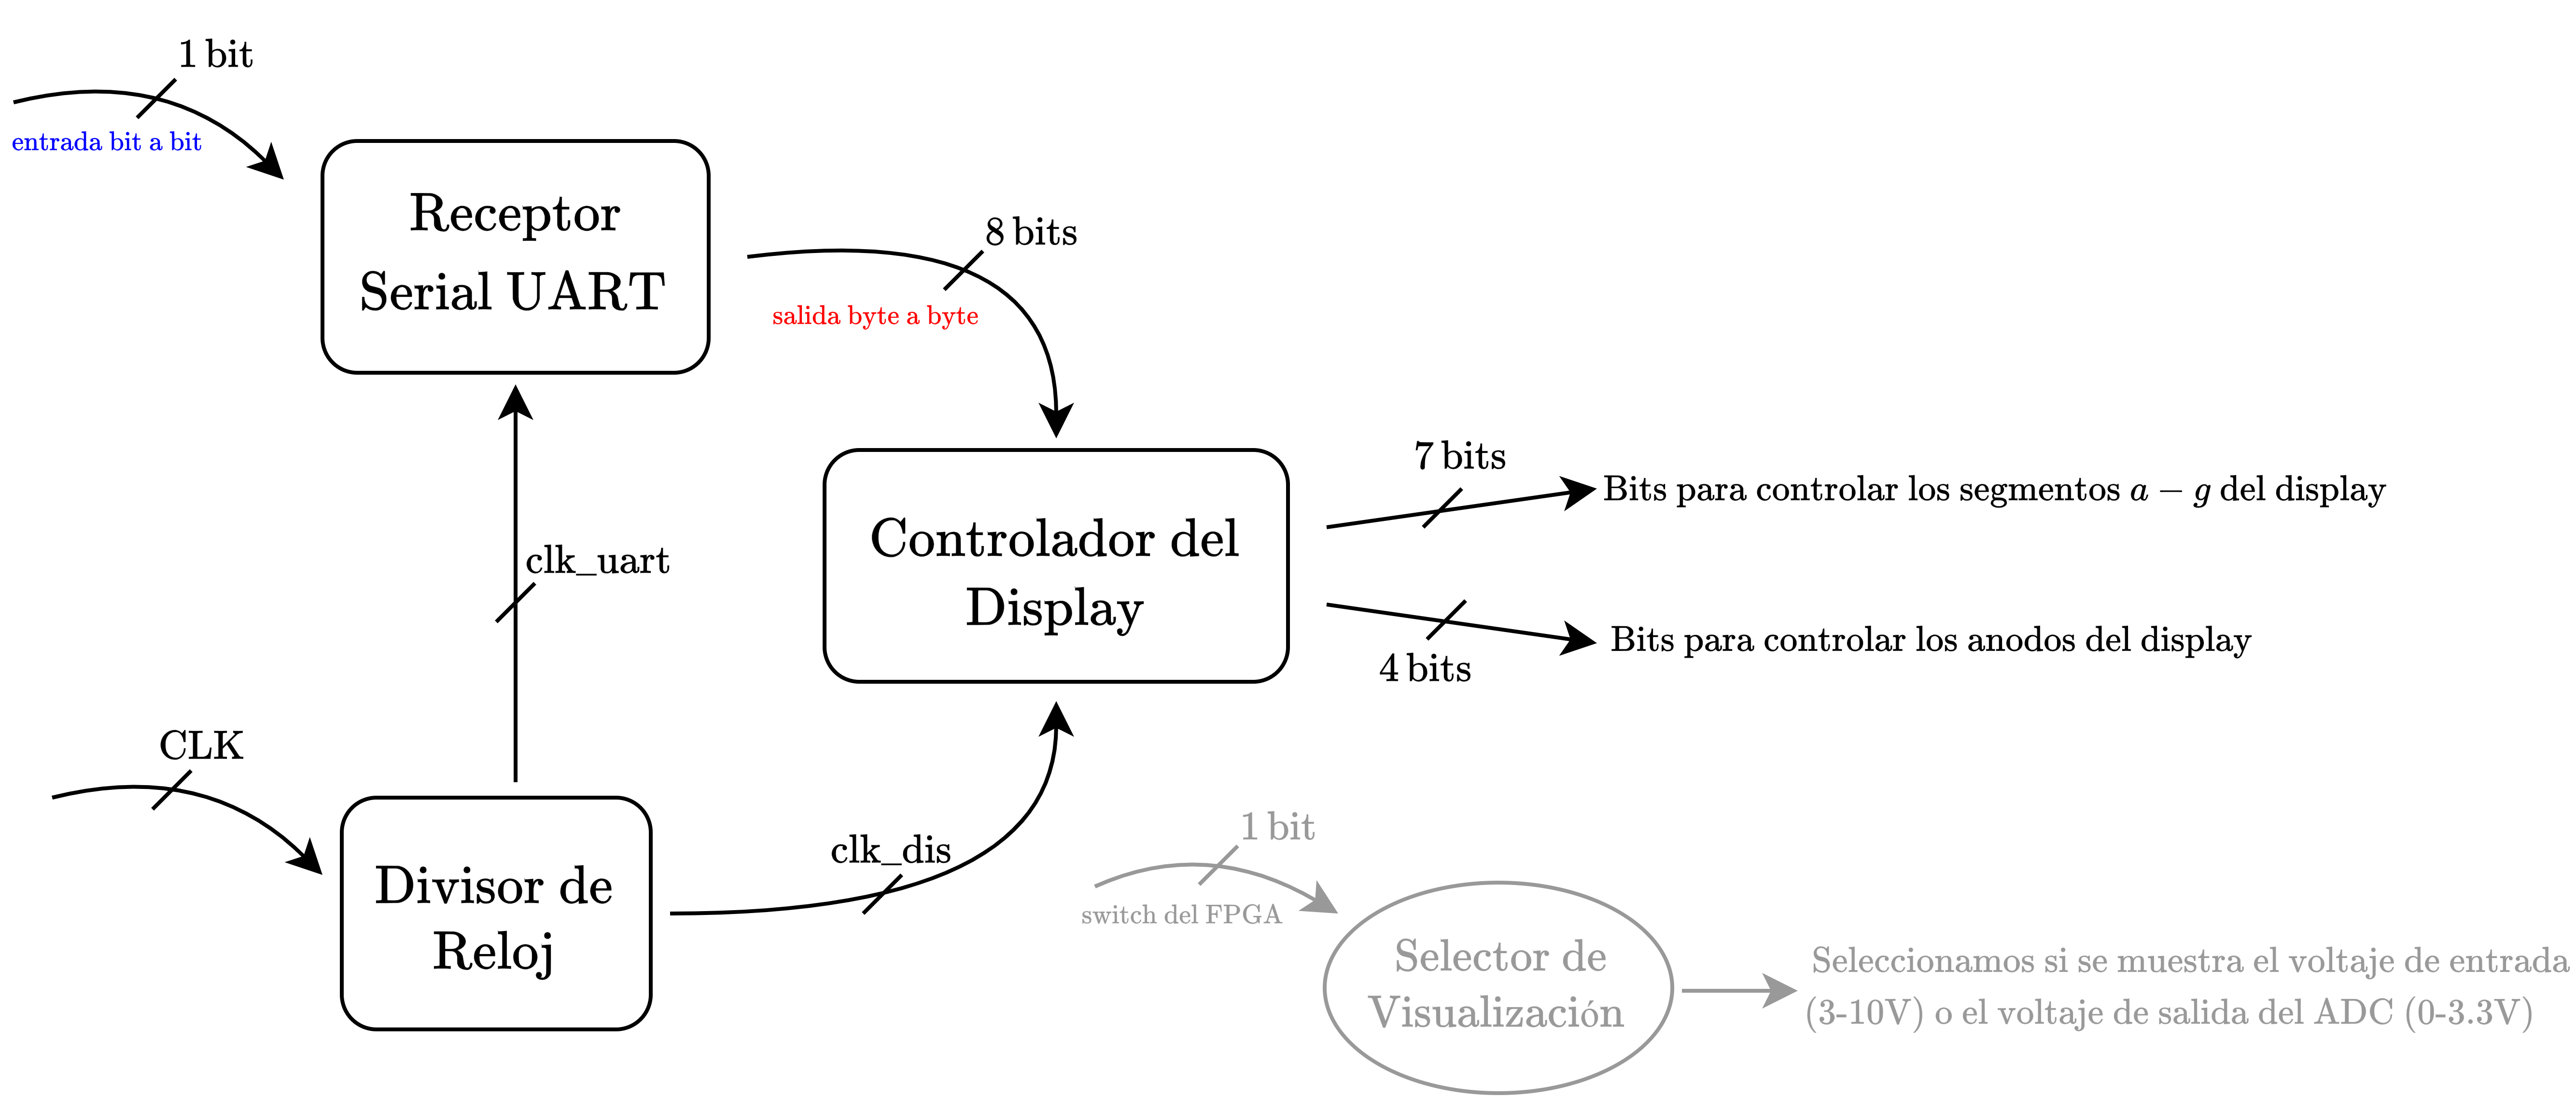
\includegraphics[width=\linewidth]{DB FPGA (Exp1).png}
    \caption{Diagrama de bloques implementación FPGA}
\end{figure}

En particular, podemos ver 4 bloques, donde 3 de ellos son los bloques principales para la implementación, mientras que el otro (el que se ve en color gris) sirve únicamente para seleccionar el voltaje que se mostrará en el display.\\

A continuación, se explica el propósito de cada bloque:

\begin{itemize}
    \item[\textbf{1.}] \textbf{Receptor Serial UART:} Para esta experiencia decidimos ocupar el protocolo de comunicación UART para generar la transmisión y recepción de datos serial desde el ESP32 a la FPGA. En este caso, las entradas del bloque son, por un lado, un CLK más lento que viene generado dividiendo el CLK de la FPGA y una entrada bit a bit serial que viene del ESP32.

    Investigando, nos dimos cuenta que el ESP32 cuando envía palabras de forma serial, las envía bit a bit, pero cada palabra que envía es de 8 bits, es decir, el proceso de comunicación serial de una palabra desde el ESP32 hasta la FPGA acaba cuando son transmitidos 8 bits (1 byte). Por esta razón es que se puede ver que la salida del bloque es un bus de 8 bits o 1 byte.

    \item[\textbf{2.}] \textbf{Divisor de Reloj:} Este bloque es fundamental para el correcto funcionamiento de la implementación. En el enunciado nos piden configurar la transmisión de datos seriales dentro del rango de 1 a 10 Kb/s, por lo que la recepción de datos de la FPGA también debe coincidir con ese rango. Por esto es que necesitamos un divisor de reloj que lleve el CLK de la FPGA (CLK de 100MHz) a un reloj que nos permita recibir datos que llegan con una velocidad de entre 1 a 10 Kb/s.

    Asi mismo, para el bloque ``Controlador de Display'' también es importante utilizar un CLK más lento, puesto que debemos enceder los leds de cada uno de los segmentos $a-g$. Si es que los encendemos y apagamos con un CLK muy rápido, la FPGA no va a poder seguir el ritmo y solo veremos una luz tenue en los segmentos.

    \item[\textbf{3.}] \textbf{Controlador del Display:} Este bloque es muy importante porque es el que nos permite tomar los bytes que vienen de la salida del ``Receptor Serial UART'' y colocar el número decimal que representan en el \textit{display} de 7 segmentos de la FPGA, con ello cumpliendo las especificaciones de la implementación.

    \item[\textbf{3.1}] \textbf{Selector de Visualización:} Tal y como se pide en las especificaciones, debemos implementar en la FPGA un switch que nos permita cambiar el número decimal que muestra el display, del voltaje en el rango de 0-3.3V al voltaje en el rango de 3-10V. Este bloque se colocó en color gris únicamente porque no será un modulo extra que se escribirá en el código, sino que es un código que ira dentro del modulo ``Controlador del Display''.
\end{itemize}

Con esto queda explicado el diagrama de bloques presentado.\\

2. Investigue las ventajas de utilizar un divisor de reloj.\\

\textbf{Respuesta:}\\

A continuación se detallan las principales ventajas que tiene utilizar un divisor de reloj particularmente en el contexto de esta experiencia:

\begin{itemize}
    \item[\textbf{1.}] \textbf{Sincornización precisa del Baud Rate:} El reloj interno de la FPGA es muy rápido (100 MHz), la comunicación UART, por otro lado, funciona a velocidades mucho menores (en nuestro caso entre 1 y 10 Kb/s). El divisor de reloj permite generar un pulso de muestreo que coinida con la velocidad de transmisión del ESP32. Necesitamos que la lógica de recepción guarde el pin de entrada en intervalos precisos para no perder la sincronización del frame.

    \item[\textbf{2.}] \textbf{Control de la persistencia en el display de 7 segmentos:} Si intentamos actualizar los dígitos del display a la velocidad del CLK de la FPGA, no podríamos ver nada debido a la velocidad de conmutación. El divisor de reloj crea una frecuencia cómoda para el ojo humano y con ello podremos ver los números que mostremos.

    \item[\textbf{3.}] \textbf{Reducción del consumo de energía:} En la FPGA, el consumo de potencia dinámica está directamente relacionado con la frecuencia de conmutación de las compuertas lógicas:
\end{itemize}
\[
P_{dynamic} \approx \sum C\cdot V^{2} \cdot f
\]
\begin{itemize}
    \item[] Si usamos relojes divididos para procesos lentos, reducimos la cantidad de transiciones por segundo, lo que mantiene a la FPGA más eficiente.

    \item[\textbf{4.}] \textbf{Estabilidad y cumplimiento de tiempos:} Hacer que toda la lógica de la FPGA corra a 100 MHz cuando solo recibimos un byte cada pocos milisegundos puede generar problemas de \textit{timing closure.} Segmentar el diseño en dominios de reloj adecuados permite que las señales tengan más tiempo para estabilizarse antes del siguiente flanco de subida, reduciendo la probabilidad de errores de metaestabilidad.
\end{itemize}

3. Escriba un código y simule un divisor de reloj.\\

\textbf{Respuesta:}\\

A continuación, se muestra el código implementado.\\

\textbf{Módulo CLK\_DIV}

\begin{lstlisting}
`timescale 1ns / 1ps

module CLK_DIV #(parameter DIV = 2)(input logic clk,       // reloj del FPGA (100 MHz)
                                    input logic rst,       // reset sincrono
                                    output logic clk_out); // reloj dividido

logic [$clog2(DIV)-1:0] count;
logic pulso;

always_ff @(posedge clk) begin
  if (rst) begin count <= '0;
                 pulso <= 1'b0;
  end else begin if (count == DIV/2 - 1) begin count <= '0;
                                               pulso <= ~pulso; end
                 else begin count <= count + 1; end
  end
end
  
assign clk_out = pulso;

endmodule
\end{lstlisting}

\textbf{Testbenche TB\_CLK\_DIV}

\begin{lstlisting}
`timescale 1ns / 1ps

module TB_CLK_DIV;

// Senales de prueba
logic clk;
logic rst;
logic clk_uart;
logic clk_display;

// Generacion de reloj de 100 MHz
initial begin clk = 0;
        forever #5 clk = ~clk; end

// Instancia 1: Reloj que se usara en el UART (153.6 kHz)
CLK_DIV #(.DIV(651)) dut_uart (.clk(clk), .rst(rst), .clk_out(clk_uart));

// Instancia 2: Reloj que se usara en el Display (0.5 kHz)
CLK_DIV #(.DIV(200000)) dut_display (.clk(clk), .rst(rst), .clk_out(clk_display));

initial begin
// Inicializacion
rst = 1; 
#20; 
rst = 0;

$finish;
end
endmodule
\end{lstlisting}

Con este código escrito y corriendo el testbenche realizado llegamos a la siguiente imagen en el simulador:

\begin{figure}[H]
    \centering
    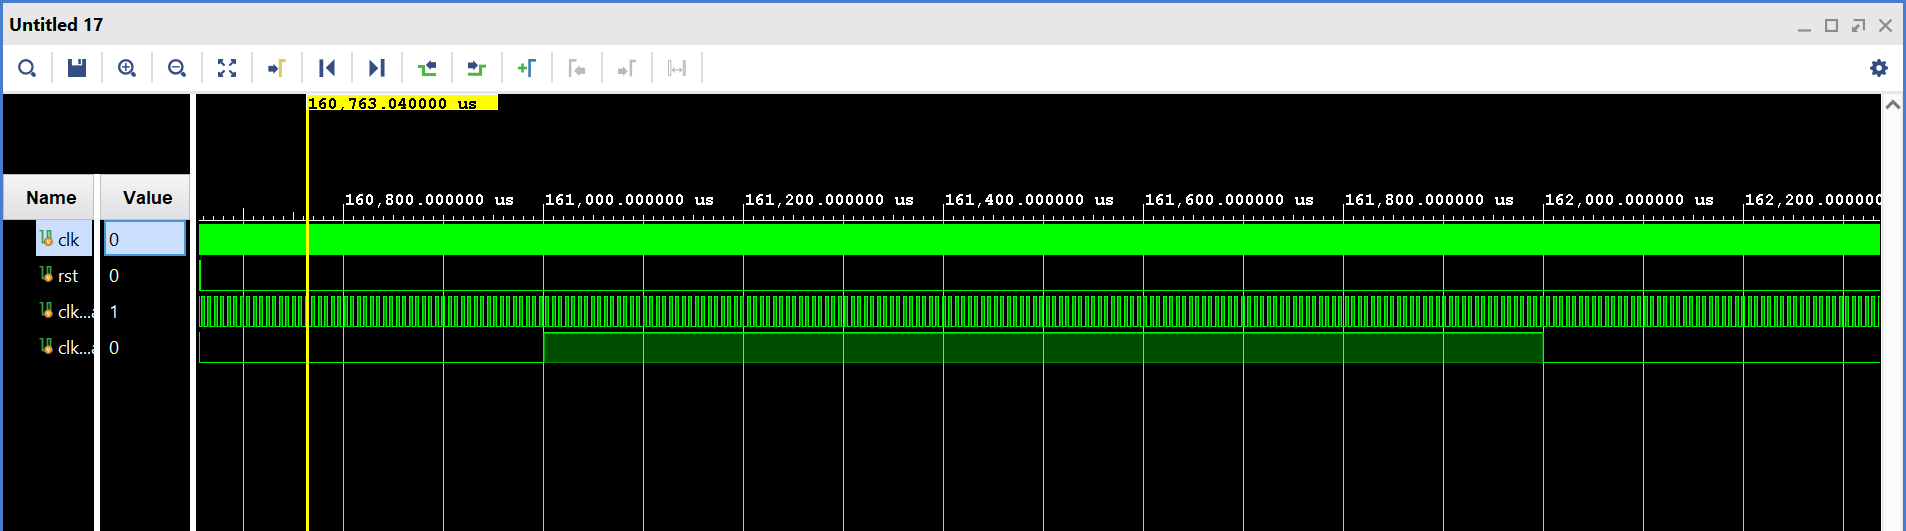
\includegraphics[width=\linewidth]{Simulación clk_divider.png}
    \caption{Simulación del divisor de reloj.}
\end{figure}

Vemos en la imagen que, efectivamente, a partir del reloj de la FPGA de 100 MHz se crean 2 relojes más lentos que luego podrán ser usados para el modulo de comunicación UART y para el modulo de la visualización en el \textit{display}.\\

4. Escriba un código y simule algún protocolo de comunicación serial.\\

\textbf{Respuesta:}\\

Cómo ya se ha mencionado antes, se opto por ocupar el protocolo de comunicación UART. A continuación se muestran el modulo y el testbenche implementado.\\

\textbf{Módulo Protocolo\_UART}

\begin{lstlisting}
`timescale 1ns / 1ps

module Protocolo_UART(
    input  logic       clk,      // Reloj principal (100MHz)
    input  logic       rst_n,    // Reset activo en bajo
    input  logic       rx,       // Entrada serial
    input  logic       clk_uart, // Reloj dividido
    output logic [7:0] data,     // Dato recibido
    output logic       done      // Pulso de finalizacion
);

// Estados de la FSM
typedef enum logic [1:0] {IDLE, START, DATA, STOP} state_type;
state_type state;

logic [3:0] tick_count; // Cuenta 16 ticks por cada bit
logic [2:0] bit_index;  // Variable que senala el bit que se esta recibiendo, 
                        // en caso de ser 7 ya se recibio todo el byte y hay 
                        // que pasar al estado STOP
logic [7:0] register;   // Variable en la que guardaremos el byte recibido

logic clk_uart_reg, clk_uart_edge;

always_ff @(posedge clk) begin
    clk_uart_reg <= clk_uart; end

assign clk_uart_edge = clk_uart && !clk_uart_reg; // Pulso de un solo ciclo de clk

always_ff @(posedge clk or negedge rst_n) begin
  if (!rst_n) begin state      <= IDLE;
                    done       <= 1'b0;
                    tick_count <= 4'b0;
                    bit_index  <= 3'b0;
                    data       <= 8'b0;
  end else begin
  if (state == IDLE) begin
     done <= 1'b0;
     if (rx == 1'b0) begin
         state      <= START;
         tick_count <= 4'b0; end
  end
                                    
  else if (clk_uart_edge) begin         // Solo opera cuando el reloj dividido da un pulso
  done <= 1'b0;
  
  case (state)
  START: if (tick_count == 7) begin     // Muestro a la mitad del bit (tick 8 de 16)
           state      <= DATA;
           tick_count <= 4'b0;
           bit_index  <= 3'b0; end
         else begin tick_count <= tick_count + 1; end
         
  DATA: if (tick_count == 15) begin     // Fin de un bit
           tick_count <= 4'b0;
           register[bit_index] <= rx;
           if (bit_index == 7) state <= STOP;
           else bit_index <= bit_index + 1; end
        else begin tick_count <= tick_count + 1; end

  STOP: if (tick_count == 15) begin     // Fin del bit de parada
           data  <= register;
           done  <= 1'b1;
           state <= IDLE; end
        else begin tick_count <= tick_count + 1; end  
  endcase
  end
end
end
endmodule
\end{lstlisting}

\textbf{Testbenche TB\_UART}

\begin{lstlisting}
`timescale 1ns / 1ps

module TB_UART;
// Senales para conectar con el DUT (Device Under Test)
logic clk;
logic rst_n;
logic rx;
logic clk_uart;
logic [7:0] data;
logic done;

// Instancia del modulo desarrollado
Protocolo_UART dut (.clk(clk), .rst_n(rst_n), .rx(rx), .clk_uart(clk_uart),
                    .data(data), .done(done));

// 1. Generador de Reloj Principal (100 MHz de la Basys 3)
initial begin clk = 0;
forever #5 clk = ~clk; end


// 2. Generador de clk_uart (Baud Tick 16x)
// Para 9600 bps: 9600 * 16 = 153.6 kHz. 
// Periodo aprox: 6510 ns -> Semi-periodo: 3255 ns
initial begin clk_uart = 0;
forever #3255 clk_uart = ~clk_uart; end

// Tarea para automatizar el envio de un byte (Emula al ESP32) [cite: 88, 154]
task send_byte(input [7:0] byte_to_send);
  integer i;
                
  // Bit de Inicio (Logica 0)
  rx = 0;
  repeat(16) @(posedge clk_uart);
        
  // 8 Bits de Datos (LSB primero como dicta el estandar)
  for (i = 0; i < 8; i = i + 1) begin
       rx = byte_to_send[i];
       repeat(16) @(posedge clk_uart); end
        
  // Bit de Parada (Logica 1)
  rx = 1;
  repeat(16) @(posedge clk_uart);
  
  repeat(5) @(posedge clk_uart);        
endtask

// 3. Estimulos de Simulacion
initial begin
// Inicializacion
rst_n = 0; rx = 1; // Linea UART en IDLE es 1
        
// Reset del sistema
#200; rst_n = 1; #200;

// Prueba 1: Enviar valor 0x3.30 (Escalado para representar voltaje) 
// Ejemplo: Enviamos 8'h02 (00000010 en binario)
send_byte(8'h02);

#500;

send_byte(8'h74);

$finish;
end
endmodule
\end{lstlisting}

El módulo implementado es una FSM (máquina de estados finita), en donde se espera el bit inicial de la palabra a recibir (el cual siempre es un 0) y a partir de ahí se comienzan a guardar los proximos 8 bits, teniendo en consideración de que debemos guardar estos bit cuando estemos en la mitad de o que demora su activación, así no tenemos errores debido a gliches o bugs. Se utiliza un CLK más lento para saber cuando guardar los bits que van llegando, luego de guardar 8 bits, la máquina de estados se reinicia y volvemos al estado IDLE esperando a que llegue un nuevo byte para leer.\\

En el testbenche se realiza la simulación de 2 palabras distintas enviadas a la FPGA, especificamente los bytes \texttt{8'h02} y \texttt{8'h74}, haciendo referencia de que el voltaje que se deberá mostrar en el display de 7 segmentos será 2.74V. Al correr la simulación obtenemos la siguiente imagen comprobando que el código funciona correctamente.

\begin{figure}[H]
    \centering
    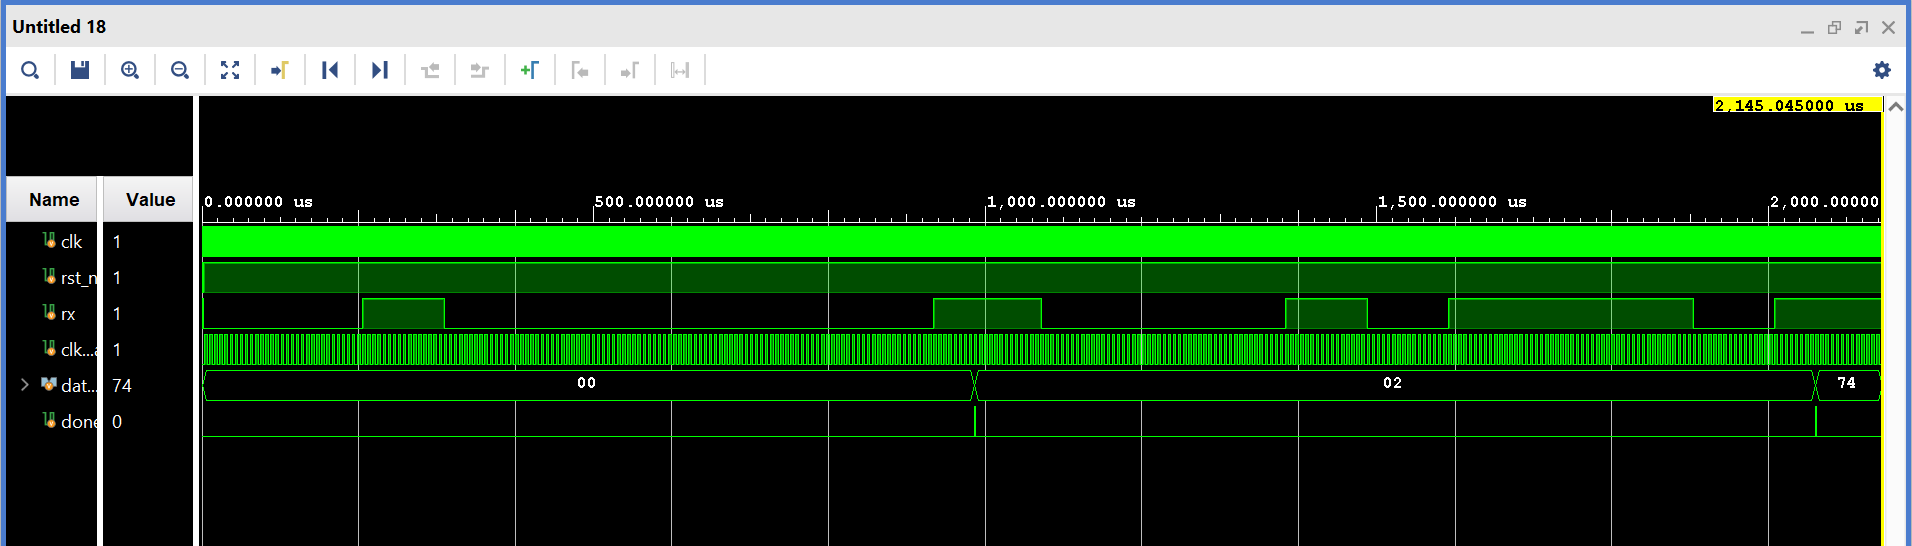
\includegraphics[width=\linewidth]{Simulación protocolo_uart.png}
    \caption{Simulación del protocolo de comunicación UART.}
\end{figure}

Vemos que la variable de salida \texttt{data} toma primero el valor de \texttt{8'h02} y luego el valor de \texttt{8'h74}, señalando de que los bytes enviados han sido recibidos exitosamente.\\
% ***********************************************
% ***********************************************
\end{document}